%Version 3.1 December 2024
%% Benchmarking multi-paradigma para avaliação integrada da qualidade do solo
%% Manuscrito PT-BR (versão de trabalho) — tradução EN ao final
%%
%%%%%%%%%%%%%%%%%%%%%%%%%%%%%%%%%%%%%%%%%%%%%%%%%%%%%%%%%%%%%%%%%%%%%%

\documentclass[pdflatex,sn-basic]{sn-jnl}% Basic Springer Nature Reference Style

%%%% Standard Packages
\usepackage{graphicx}%
\usepackage{multirow}%
\usepackage{amsmath,amssymb,amsfonts}%
\usepackage{amsthm}%
\usepackage{mathrsfs}%
\usepackage[title]{appendix}%
\usepackage{xcolor}%
\usepackage{textcomp}%
\usepackage{manyfoot}%
\usepackage{booktabs}%
\usepackage{algorithm}%
\usepackage{algorithmicx}%
\usepackage{algpseudocode}%
\usepackage{listings}%
\usepackage{tikz}%
\usepackage{subcaption}%

\raggedbottom

\begin{document}

\title[Paradigma estatístico e qualidade do solo]{Escolha do paradigma estatístico como condicionante para avaliação de qualidade do solo em Argissolo sob manejo conservacionista de longa duração}

%%=============================================================%%
%% Autores
%%=============================================================%%

\author*[1]{\fnm{Luiz Diego Vidal} \sur{Santos}}\email{ldvsantos@uefs.br}

\author[2]{\fnm{Alceu} \sur{Pedrotti}}\email{alceu.pedrotti@instituicao.edu.br}

\author[1]{\fnm{Autor3\_Nome} \sur{Autor3\_Sobrenome}}\email{autor3@instituicao.edu.br}

\affil*[1]{\orgdiv{Departamento}, \orgname{Instituição}, \orgaddress{\city{Cidade}, \state{Estado}, \country{Brasil}}}

\affil[2]{\orgdiv{Departamento}, \orgname{Instituição}, \orgaddress{\city{Cidade}, \state{Estado}, \country{Brasil}}}

%%==================================%%
%% Resumo
%%==================================%%

\abstract{Índices de qualidade do solo (IQS) são geralmente construídos por um único paradigma estatístico, o que impede a comparação direta entre abordagens e pode conduzir a conclusões dependentes do método adotado. Este estudo tem por objetivo investigar em que medida a escolha do paradigma estatístico altera a avaliação integrada de qualidade do solo, quantificando concordância e discordância entre cinco abordagens analíticas de famílias estruturalmente distintas (ANOVA/GLM, SIF, PLS-SEM, MARS e RF) aplicadas ao mesmo conjunto de dados ($n = 108$, 15 indicadores, três sistemas de manejo e quatro espécies de cobertura em experimento de 22 anos). O coeficiente de concordância de Kendall ($W = 0{,}81$) e o coeficiente de correlação intraclasse ($\text{ICC} = 0{,}72$) indicaram concordância elevada entre os cinco ranqueamentos simultâneos, embora com estrutura em três camadas de intensidade. Inferência fuzzy, MARS e \textit{Random Forest} formaram bloco praticamente intercambiável, o PLS-SEM ocupou posição intermediária e a ANOVA divergiu de todos os demais, com diferenças suficientes para inverter posições intermediárias do ranqueamento de manejo. O cultivo mínimo com feijão-guandu concentrou os maiores escores de qualidade em todos os paradigmas. Simulações Monte Carlo indicaram que a concordância se estabiliza acima de aproximadamente 50 observações. Os resultados sugerem que os paradigmas não lineares (SIF, MARS e RF) podem substituir-se mutuamente sem perda prática de informação, ao passo que comparações envolvendo o paradigma linear (ANOVA/GLM) requerem verificação de sensibilidade ao método.}

\keywords{índice de qualidade do solo, sistema de inferência fuzzy, PLS-SEM, MARS, Random Forest, ANOVA, comparação metodológica, plantas de cobertura, sistemas de manejo}

\maketitle

%% ================================================================
%%                    SEÇÃO 1: INTRODUÇÃO
%% ================================================================
\section{Introdução}\label{sec:intro}

A degradação do solo compromete a capacidade produtiva de aproximadamente 33\% das terras agrícolas globais, com perdas anuais estimadas entre 25 e 40 bilhões de toneladas de solo fértil por erosão hídrica e eólica \cite{Lal2015}. Nos trópicos úmidos, onde a mineralização acelerada da matéria orgânica e a agressividade das chuvas intensificam esses processos, a adoção de sistemas conservacionistas (plantio direto, cultivo mínimo e uso de plantas de cobertura) tornou-se estratégia central para a manutenção das funções edáficas \cite{Doran2002,Cardoso2013}. A avaliação quantitativa da eficácia dessas práticas requer ferramentas que integrem atributos físicos, químicos e biológicos em métricas auditáveis, o que motivou o desenvolvimento dos índices de qualidade do solo (IQS) \cite{Karlen1997}.

O conceito de IQS consolidou-se a partir do arcabouço proposto por \cite{Karlen1997} e do protocolo operacional de \cite{Andrews2002}, que estabeleceu a seleção de conjunto mínimo de dados (MDS) por análise de componentes principais (ACP) seguida de escorificação aditiva. Desde então, revisões abrangentes documentaram a proliferação de variantes metodológicas, com mais de 60 combinações de seleção, ponderação e agregação publicadas até 2018 \cite{Bünemann2018}. Essa diversidade, embora sinal de maturidade da área, introduz um problema de comparabilidade entre estudos que adotam paradigmas distintos para os mesmos indicadores.

Na abordagem clássica, modelos paramétricos (ANOVA ou GLM) produzem escores lineares a partir de pesos derivados de autovalores da ACP, supondo que as relações entre indicadores e qualidade do solo são monotônicas e aditivas \cite{Mukherjee2014}. A simplicidade computacional e a transparência interpretativa tornaram esse paradigma predominante em avaliações de manejo conservacionista, inclusive em experimentos de longa duração sobre Argissolos dos Tabuleiros Costeiros do Nordeste brasileiro \cite{Assuncao2023}. A limitação reside na incapacidade do modelo linear de capturar efeitos limiares e interações de ordem superior entre indicadores de domínios distintos \cite{DosSantos2021}.

Sistemas de inferência fuzzy (SIF) foram introduzidos como alternativa para acomodar a incerteza de fronteira inerente à classificação de indicadores contínuos em categorias discretas de qualidade \cite{Torbert2008}. Ao substituir cortes rígidos por funções de pertinência triangulares ou gaussianas, o SIF preserva a gradação dos atributos edáficos e permite a incorporação de conhecimento especializado por meio de bases de regras linguísticas \cite{Nabiollahi2018}. Aplicações recentes em solos tropicais brasileiros indicaram que o SIF pode detectar diferenças de manejo que o protocolo aditivo clássico não distingue \cite{DosSantos2021}, embora a calibração das funções de pertinência permaneça dependente de dados regionais nem sempre disponíveis.

Algoritmos de aprendizado de máquina (AM), a exemplo de \textit{Random Forest} (RF) e \textit{Multivariate Adaptive Regression Splines} (MARS), exploram não linearidade e interação de alta ordem por meio de particionamento recursivo do espaço de preditores \cite{Zeraatpisheh2020}. O RF, em particular, oferece métricas intrínsecas de importância de variáveis (por permutação ou impureza) e estimativas \textit{out-of-bag} que dispensam validação cruzada explícita, o que o tornou popular em mapeamento digital de solos \cite{Wadoux2020}. O MARS, por sua vez, identifica limiares (\textit{knots}) adaptativos que aproximam descontinuidades na resposta sem recorrer à discretização prévia dos indicadores. A interpretabilidade do AM, porém, é inferior à dos modelos estatísticos clássicos, e o risco de sobreajuste em amostras pequenas ($n < 50$) requer atenção \cite{Chaudhry2024}.

A modelagem de equações estruturais por mínimos quadrados parciais (PLS-SEM) ocupa posição intermediária entre os paradigmas anteriores. Ao especificar construtos latentes que representam domínios edáficos (físico, agronômico, rendimento) e estimar coeficientes de caminho entre eles, o PLS-SEM testa hipóteses causais sobre a cadeia solo--planta--rendimento \cite{Hair2019,Sarstedt2022}. A especificação mista (Mode~A reflexivo para indicadores que manifestam o construto e Mode~B formativo para indicadores que causam o construto) confere flexibilidade teórica \cite{Diamantopoulos2008}, embora a linearidade dos caminhos estruturais limite a captura de interações não lineares entre domínios.

Na prática, cada estudo opta por um único paradigma e assume, implicitamente, que o ranqueamento das combinações de manejo é estável frente à escolha metodológica. Comparações recentes envolvendo variantes de escorificação \cite{Mukherjee2014}, aprendizado de máquina \cite{Chaudhry2024} e lógica fuzzy--AHP \cite{Pacci2026} abordaram o problema, porém restringiram-se a duas ou três abordagens da mesma família analítica e não empregaram métricas formais de concordância inter-avaliador \cite{Venkateswarlu2025,Liu2025}. 

Permanece, portanto, sem resposta a pergunta sobre em que medida a escolha do paradigma altera conclusões de manejo quando famílias estruturalmente distintas são confrontadas simultaneamente.

Os Argissolos dos Tabuleiros Costeiros do Nordeste brasileiro, derivados de sedimentos da Formação Barreiras, apresentam horizonte A franco-arenoso e camada coesa em subsuperfície que limita a drenagem interna e a penetração radicular \cite{LimaNeto2010}. Nessas condições, experimentos de longa duração demonstraram que sistemas conservacionistas melhoram indicadores físicos e biológicos, ainda que lentamente, produzindo gradientes de qualidade entre combinações manejo--cobertura que tendem a ser sutis \cite{Assuncao2023,Oliveira2020,Lopes2021}. Se os paradigmas estatísticos divergem justamente nesses gradientes sutis, as recomendações de manejo derivadas de um IQS passam a ser contingentes ao método, comprometendo a reprodutibilidade e a utilidade prática do índice.

Este estudo tem por objetivo investigar em que medida a escolha do paradigma estatístico altera a avaliação integrada de qualidade do solo, quantificando concordância e discordância entre cinco abordagens analíticas de famílias estruturalmente distintas (ANOVA/GLM, SIF, PLS-SEM, MARS e RF) aplicadas ao mesmo conjunto de dados ($n = 108$, 15 indicadores, três sistemas de manejo e quatro espécies de cobertura em experimento de 22 anos). Três hipóteses direcionais orientam a investigação: ($H_1$) os paradigmas produzem concordância de ranqueamento estatisticamente diferente de zero ($W > 0$, $\alpha = 0{,}05$); ($H_2$) métodos não lineares (SIF, MARS, RF) exibem maior convergência mútua do que com o paradigma linear (GLM); e ($H_3$) a concordância inter-paradigma cresce log-linearmente com o tamanho amostral até estabilizar a partir de $n \approx 75$.

%% ================================================================
%%                    SEÇÃO 2: MATERIAL E MÉTODOS
%% ================================================================
\section{Material e Métodos}\label{sec:material}

\subsection{Descrição do conjunto de dados}\label{subsec:dataset}

O conjunto de dados utilizado neste \textit{benchmarking} foi obtido em experimento de campo de longa duração conduzido na Estação Experimental da Universidade Federal de Sergipe, município de São Cristóvão, SE (10$^\circ$55$'$24$''$\,S, 37$^\circ$11$'$57$''$\,W, 22\,m de altitude), conforme ilustrado na Fig.~\ref{fig:site}. O clima regional é classificado como As$'$ (tropical chuvoso com verão seco) segundo Köppen, com precipitação anual de aproximadamente 1\,600\,mm concentrada entre abril e setembro. O solo é um Argissolo Vermelho Amarelo Distrófico (\textit{Acrisol}, WRB; \textit{Typic Hapludult}, USDA), derivado da Formação Barreiras, com horizonte A franco-arenoso e presença de camada coesa em subsuperfície. O experimento foi instalado em 2001 em delineamento de faixas subdivididas (\textit{strip-split plot}) com subparcelas de 6\,m\,$\times$\,10\,m, e os dados analisados correspondem ao 22$^\circ$ ano de condução contínua (safra 2022). A avaliação do IQS pelo método aditivo clássico, referente ao 17$^\circ$ ano desse experimento, foi publicada por \cite{Assuncao2023}; o presente estudo amplia essa base ao aplicar cinco paradigmas analíticos à safra 2022.

\begin{figure}[ht]
\centering
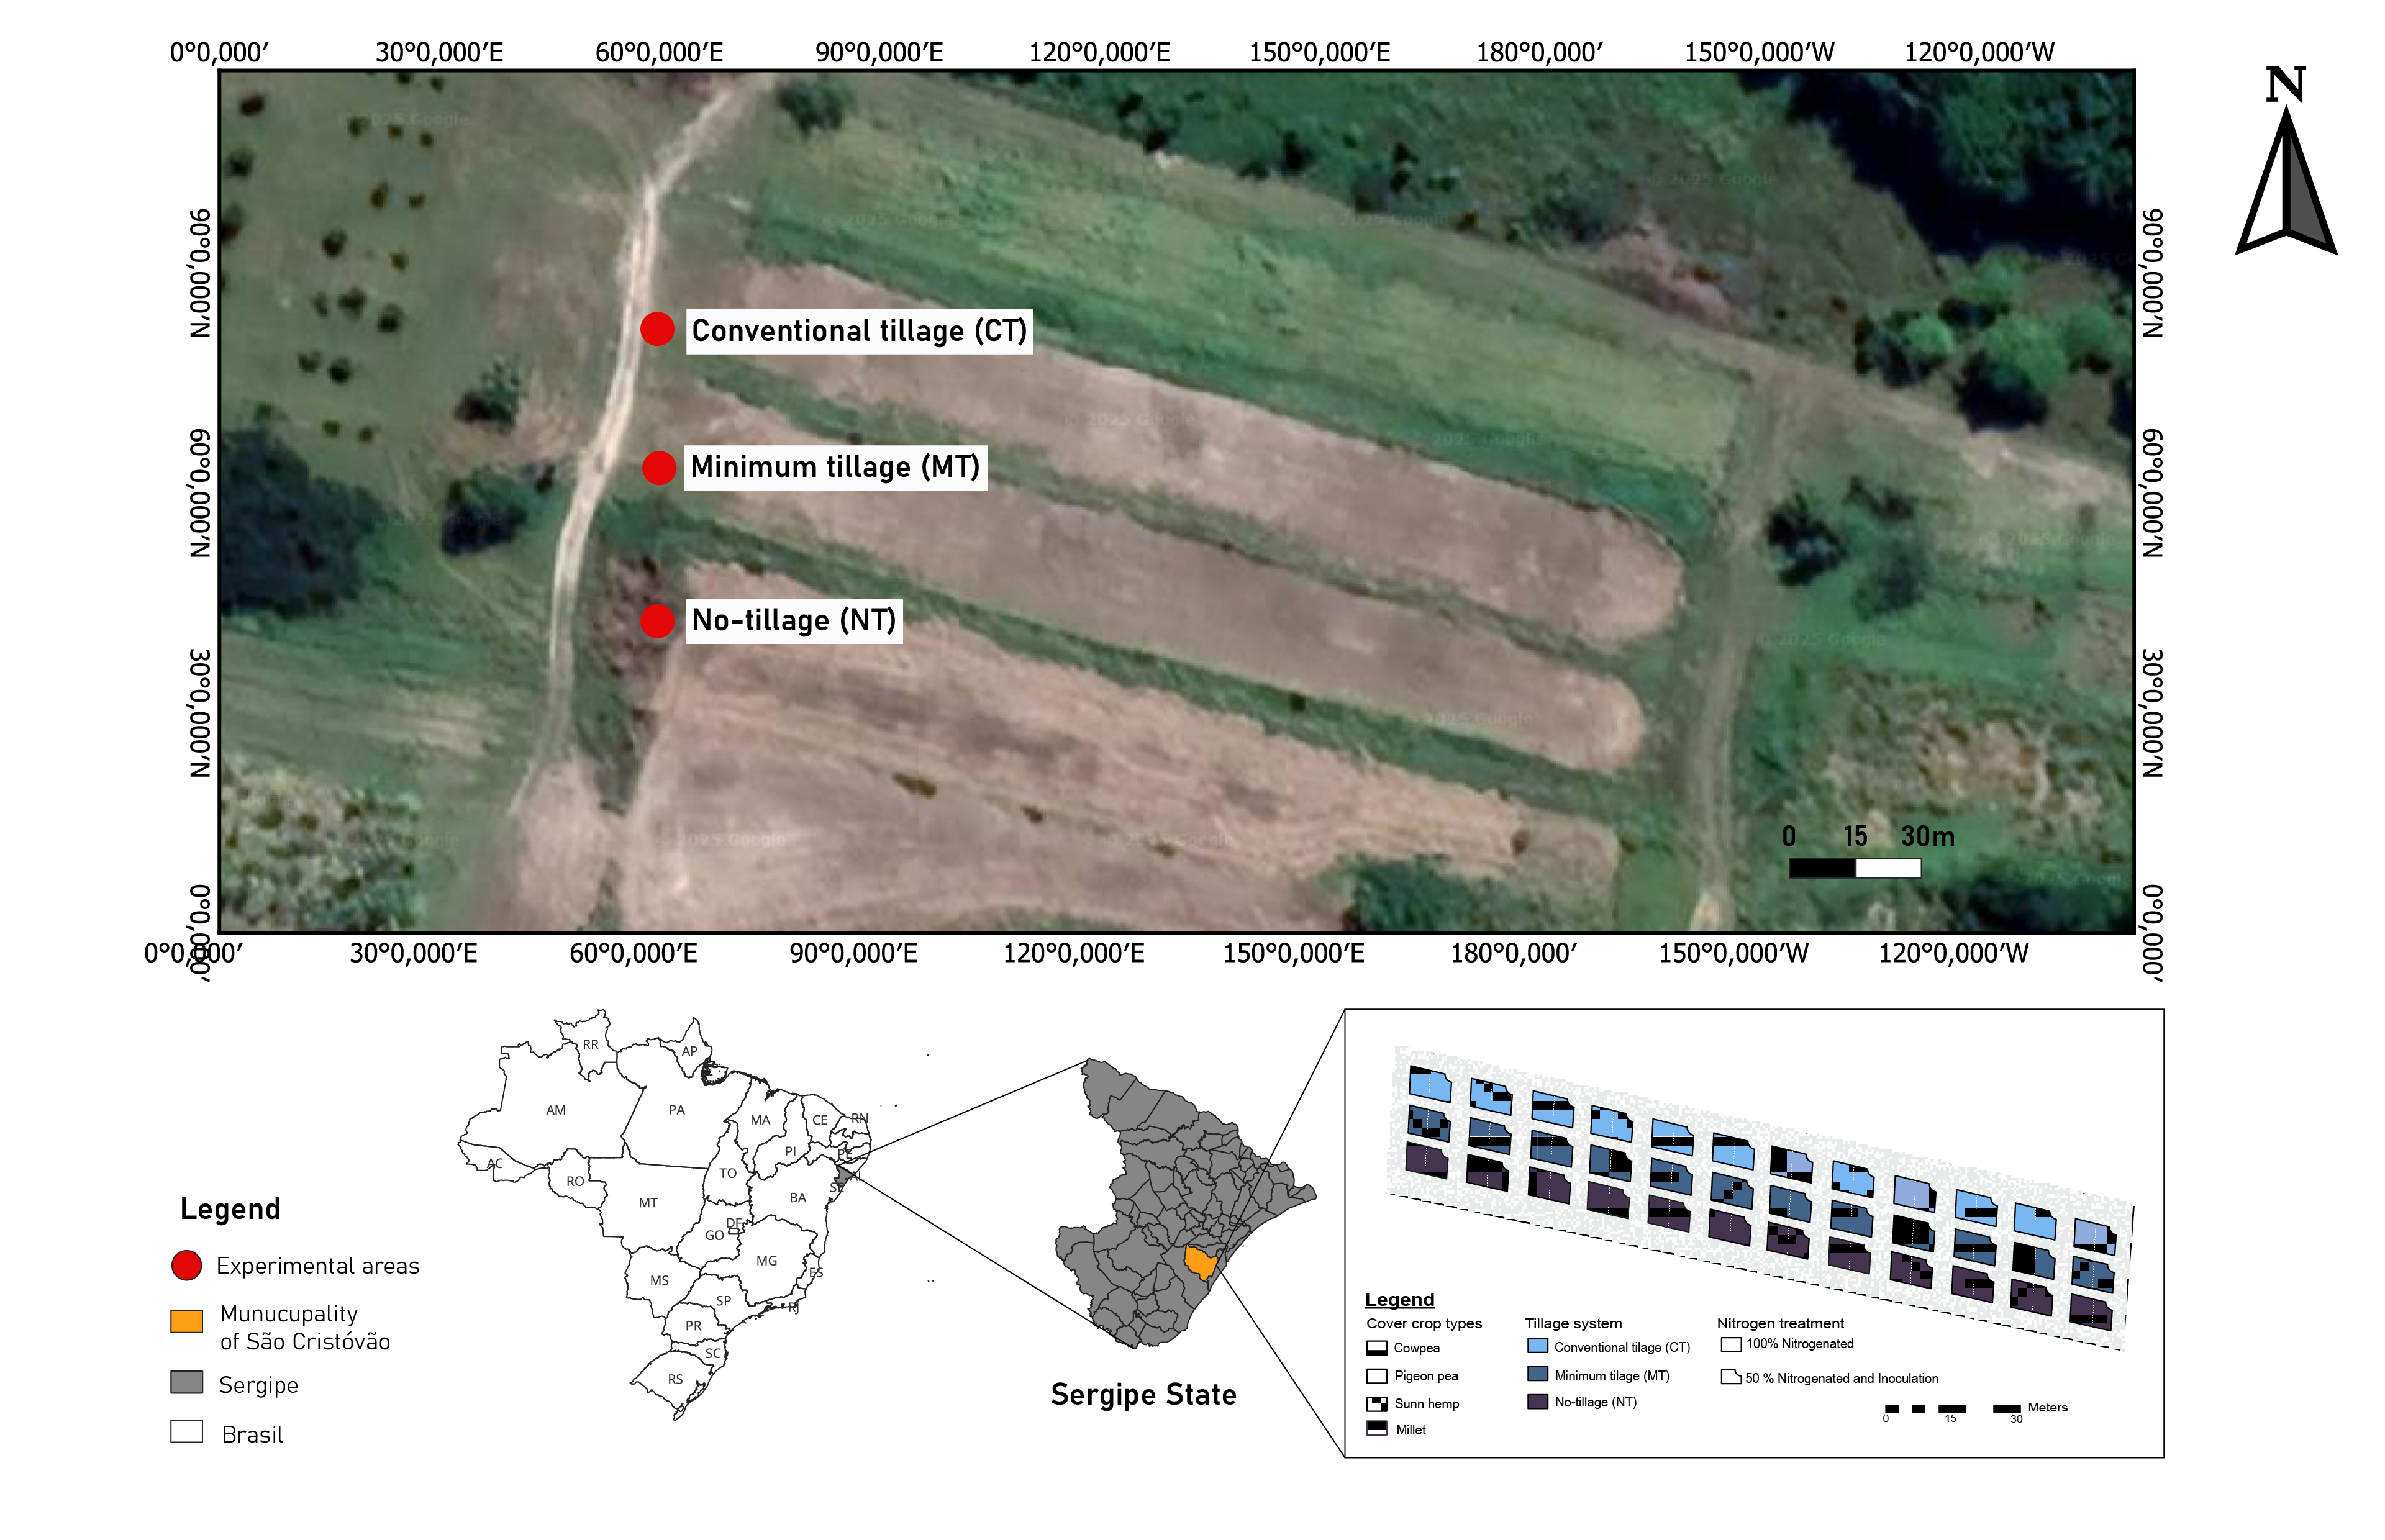
\includegraphics[width=0.85\textwidth]{../../2-DADOS/3-FIGURAS/fig_experimental_site.jpg}
\caption{Localização e vista geral do experimento de longa duração (implantado em 2001) na Estação Experimental da Universidade Federal de Sergipe, município de São Cristóvão, SE, sobre Argissolo Vermelho Amarelo Distrófico dos Tabuleiros Costeiros.}\label{fig:site}
\end{figure}

As observações ($n = 108$) foram coletadas em delineamento fatorial que combinou três sistemas de manejo do solo (plantio direto, PD; plantio convencional, PC; e cultivo mínimo, CM) com quatro espécies de plantas de cobertura (feijão-caupi, \textit{Vigna unguiculata}; milheto, \textit{Pennisetum glaucum}; feijão-guandu, \textit{Cajanus cajan}; e crotalária, \textit{Crotalaria juncea}), totalizando 12 combinações com nove repetições cada. A cultura principal \textit{Zea mays} L. (híbrido SHS7990 PRO3) foi semeada no espaçamento de 0,80\,m\,$\times$\,0,20\,m ($\approx$\,54\,000\,plantas\,ha$^{-1}$), precedida pela cobertura semeada manualmente 90 dias antes. O plantio convencional consistiu em aração com disco a 25\,cm seguida de grade niveladora, o cultivo mínimo empregou apenas grade niveladora e o plantio direto dispensou revolvimento mecânico.

\subsection{Indicadores de solo e planta}\label{subsec:indicators}

Quinze indicadores que abrangem os domínios físico do solo, agronômico e de rendimento foram mensurados (Tabela~\ref{tab:indicators}).

\begin{table}[h]
\caption{Indicadores de solo e planta utilizados na análise de \textit{benchmarking}.}\label{tab:indicators}
\begin{tabular*}{\textwidth}{@{\extracolsep\fill}llll}
\toprule
Domínio & Indicador & Sigla & Unidade \\
\midrule
\multirow{7}{*}{Físico do solo} 
  & Diâmetro médio geométrico & DMG & mm \\
  & Diâmetro médio ponderado & DMP & mm \\
  & Densidade do solo & Ds & Mg\,m$^{-3}$ \\
  & Persistência de umidade residual & RMP & -- \\
  & Agregados estáveis em água & Na & \% \\
  & Estoque de carbono orgânico do solo & COS & Mg\,ha$^{-1}$ \\
  & Índice de cobertura vegetal & ICV & \% \\
\midrule
\multirow{4}{*}{Agronômico} 
  & Altura de plantas & ALT & cm \\
  & Diâmetro da espiga & DESP & mm \\
  & Comprimento da espiga & CESP & cm \\
  & Estande final & STAND & plantas\,ha$^{-1}$ \\
\midrule
\multirow{4}{*}{Rendimento} 
  & Número total de espigas por hectare & NESP & espigas\,ha$^{-1}$ \\
  & Espigas comerciais por hectare & NESPC & espigas\,ha$^{-1}$ \\
  & Peso de espigas comerciais por hectare & PESP & kg\,ha$^{-1}$ \\
  & Índice de qualidade arquitetural & ARQ & -- \\
\botrule
\end{tabular*}
\smallskip\noindent\textit{Nota:} Todos os indicadores foram normalizados para a escala 0--10 previamente à aplicação dos paradigmas fuzzy e de AM.
\end{table}

\subsection{Paradigma 1: ANOVA/GLM com seleção de conjunto mínimo de dados}\label{subsec:anova}

A abordagem clássica seguiu o protocolo de \cite{Andrews2002}. Modelos lineares generalizados (GLM) foram ajustados para cada indicador conforme
\begin{equation}
Y_{ijk} = \mu + \alpha_i + \beta_j + (\alpha\beta)_{ij} + \varepsilon_{ijk}
\label{eq:glm}
\end{equation}
em que $\alpha_i$ representa o efeito do sistema de manejo ($i = 1, 2, 3$), $\beta_j$ o efeito da espécie de cobertura ($j = 1, \ldots, 4$), $(\alpha\beta)_{ij}$ a interação entre ambos e $\varepsilon_{ijk}$ o erro residual. A ANOVA tipo~II foi processada com o pacote \texttt{car}. Comparações múltiplas entre médias foram realizadas por médias marginais estimadas (\texttt{emmeans}) com ajuste de Tukey.

A seleção de conjunto mínimo de dados (MDS) foi conduzida via ACP. Indicadores com cargas fatoriais superiores a 0,70 em cada componente retido foram identificados e, dentre indicadores correlacionados dentro de cada componente, aquele com maior comunalidade foi retido. O IQS linear foi computado como
\begin{equation}
\text{IQS}_{\text{ANOVA}} = \sum_{i=1}^{k} w_i \cdot S_i
\label{eq:sqi_anova}
\end{equation}
em que $w_i$ corresponde ao peso derivado dos autovalores da ACP e $S_i$ ao escore normalizado de cada indicador.

\subsection{Paradigma 2: Sistema de inferência fuzzy}\label{subsec:fuzzy}

Um sistema de inferência fuzzy do tipo Mamdani foi construído segundo o arcabouço de \cite{Torbert2008}. Cada um dos 15 indicadores foi fuzzificado em três categorias linguísticas (baixo, médio, alto) com funções de pertinência triangulares e, separadamente, gaussianas. As funções triangulares foram definidas como
\begin{equation}
\mu_A(x) = \max\left(\min\left(\frac{x-a}{b-a},\; \frac{c-x}{c-b}\right),\; 0\right)
\label{eq:trimf}
\end{equation}
em que $a$, $b$ e $c$ delimitam o suporte e o pico do conjunto fuzzy. As funções gaussianas seguiram
\begin{equation}
\mu_A(x) = \exp\left(-\frac{(x-c)^2}{2\sigma^2}\right)
\label{eq:gaussmf}
\end{equation}

A base de regras foi elaborada a partir de conhecimento especializado e a defuzzificação realizada pelo método do centróide. A saída, denominada Índice de Performance e Conservação do Solo Integrado (IPACSA), foi computada na escala 0--10 com o pacote \texttt{FuzzyR}.

\subsection{Paradigma 3: Modelagem de equações estruturais PLS-SEM}\label{subsec:sem}

Um modelo de caminhos PLS hierárquico foi especificado com três construtos latentes de primeira ordem (FÍSICO, AGRONÔMICO e RENDIMENTO) e um construto de segunda ordem, IQS. O modelo estrutural especificou caminhos direcionais conforme
\begin{equation}
\text{IQS}_{\text{PLS}} = \gamma_1 \cdot \eta_{\text{FIS}} + \gamma_2 \cdot \eta_{\text{AGRO}} + \gamma_3 \cdot \eta_{\text{REND}} + \zeta
\label{eq:plssem}
\end{equation}
Indicadores como densidade do solo (Ds) e produção de espigas (PESP, NESPC) atuam como causas (e não como reflexos) de seus respectivos construtos, o que implica relações formativas. Por essa razão, o modelo adotou especificação mista (Mode~A para indicadores reflexivos e Mode~B para indicadores formativos), conforme recomendado por \cite{Hair2019}. Quatro indicadores com VIF\,$> 5$ (DMP, RMP, Ds, NESPC) foram excluídos previamente à estimação para evitar singularidade da matriz de correlação, resultando em 11 indicadores distribuídos entre os três construtos de primeira ordem. A validação de Mode~B seguiu critérios de significância dos pesos externos (\textit{outer weights}) e ausência de multicolinearidade residual.

A estimação seguiu abordagem em dois estágios (\textit{two-stage approach}) com o pacote \texttt{seminr} \cite{Ray2022}. No primeiro estágio, os três construtos de primeira ordem (FÍSICO, AGRO, REND) foram estimados iterativamente, com caminhos estruturais FÍSICO$\to$REND e AGRO$\to$REND. No segundo estágio, os escores latentes dos três construtos foram submetidos a ACP, e o primeiro componente principal foi adotado como IQS$_{\text{PLS}}$, escalado para o intervalo 0--10. Intervalos de confiança dos coeficientes de caminho foram obtidos por \textit{bootstrap} de 5\,000 reamostras.

\subsection{Paradigma 4: MARS com análise de ablação}\label{subsec:mars}

Modelos MARS foram ajustados com o pacote \texttt{earth} \cite{Milborrow2023} para capturar relações não lineares entre indicadores e uma variável-alvo (rendimento ou IQS composto). O modelo selecionou funções-base por adição progressiva (\textit{forward stepwise}) e poda reversa (\textit{backward pruning}) conforme
\begin{equation}
\hat{f}(x) = \beta_0 + \sum_{m=1}^{M} \beta_m \prod_{k=1}^{K_m} h_{km}(x_{v(k,m)})
\label{eq:mars}
\end{equation}
em que $h_{km}$ são funções-dobradiça (\textit{hinge}) da forma $\max(0, x - t)$ ou $\max(0, t - x)$.

A importância das variáveis foi avaliada por análise de ablação, na qual cada indicador foi sequencialmente removido e o deslocamento absoluto médio do ranqueamento (\textit{Mean Absolute Rank Shift}) quantificou o impacto sobre o IQS predito. Indicadores cujo escore de ablação superou um limiar pré-definido foram classificados como insubstituíveis para o índice. Adicionalmente, a importância global das variáveis foi estimada por valores SHAP (\textit{SHapley Additive exPlanations}) com o pacote \texttt{DALEX}, possibilitando comparação direta com as métricas de importância do RF e alinhamento interpretativo entre paradigmas.

\subsection{Paradigma 5: Regressão por \textit{Random Forest}}\label{subsec:rf}

Modelos de \textit{Random Forest} foram treinados com o pacote \texttt{randomForest} utilizando 500 árvores, $\lfloor \sqrt{p} \rfloor = 4$ variáveis amostradas aleatoriamente em cada divisão e tamanho mínimo de nó terminal igual a~5. A escolha de $\text{mtry} = \lfloor \sqrt{p} \rfloor$ em vez de $\lfloor p/3 \rfloor$ reduz a correlação entre árvores e confere maior estabilidade ao \textit{ensemble} quando a razão $n/p$ é moderada ($\approx 7{,}2$). A convergência do erro \textit{out-of-bag} (OOB-MSE) foi verificada por meio de curva OOB-MSE $\times$ número de árvores, e estimativas de erro OOB forneceram métrica interna de validação. A importância das variáveis foi quantificada por duas vias complementares, o incremento percentual no erro quadrático médio (\%IncMSE) após permutação de cada preditor e valores SHAP globais obtidos com o pacote \texttt{DALEX} (500 permutações). Intervalos de confiança a 95\% para as predições de IQS foram estimados pelo método \textit{infinitesimal jackknife} implementado no pacote \texttt{randomForestCI}. O IQS predito foi definido como
\begin{equation}
\text{IQS}_{\text{RF}} = \frac{1}{B}\sum_{b=1}^{B} T_b(\mathbf{x})
\label{eq:rf}
\end{equation}
em que $T_b$ corresponde à predição da árvore $b$ para a observação $\mathbf{x}$.

\subsection{Avaliação da concordância inter-paradigma}\label{subsec:concordance}

Os cinco paradigmas geram valores de IQS em escalas distintas. Previamente à comparação, todos os vetores de IQS foram padronizados pela transformação normal inversa baseada em postos \cite{Blom1958}, conforme
\begin{equation}
z_i = \Phi^{-1}\!\left(\frac{r_i - 0{,}5}{n}\right)
\label{eq:blom}
\end{equation}
em que $r_i$ é o posto da observação $i$ e $\Phi^{-1}$ a função quantil da distribuição normal padrão. Essa transformação preserva a ordenação original e coloca todos os paradigmas em escala gaussiana padrão, eliminando distorções oriundas de diferenças de domínio (0--1 vs.\ 0--10 vs.\ escores fatoriais).

A concordância entre paradigmas foi avaliada por cinco métricas complementares. O coeficiente de concordância de Kendall ($W$) quantificou o grau de acordo não paramétrico entre os cinco ranqueamentos simultâneos, variando de $W = 0$ (ausência de acordo) a $W = 1$ (acordo perfeito), com significância avaliada por teste de permutação (10\,000 repetições). O coeficiente de correlação intraclasse, ICC(2,1), avaliou a concordância absoluta entre paradigmas tratados como avaliadores independentes. O coeficiente AC2 de Gwet \cite{Gwet2008} foi calculado como métrica de concordância adicional, por ser mais estável que $W$ quando o número de avaliadores é reduzido ($k \leq 10$), utilizando o pacote \texttt{irrCAC}. A análise de Bland--Altman gerou, para cada par de paradigmas, gráficos da diferença ($\text{IQS}_A - \text{IQS}_B$) versus a média de ambos, com limites de concordância a $\pm 1{,}96$ desvios-padrão. Adicionalmente, uma matriz de correlação de Spearman ($\rho$) foi computada entre os cinco vetores padronizados de IQS. Para fins práticos, um meta-IQS foi obtido pela média dos postos (\textit{Borda count}) dos cinco paradigmas \cite{Lin2010}, agregando a informação de todos os métodos em uma única métrica ordinal.

O teste de $H_2$ (maior concordância entre paradigmas não lineares) foi conduzido por Wilcoxon pareado sobre os valores de $\rho$ transformados por Fisher-$Z$, comparando o subconjunto de pares não-linear$\times$não-linear com os pares linear$\times$não-linear.

\subsection{Sensibilidade ao tamanho amostral}\label{subsec:sensitivity}

A robustez dos paradigmas sob amostras reduzidas foi avaliada por reamostragem Monte Carlo estratificada. O conjunto completo ($n = 108$) foi subamostrado em cinco níveis ($n = 15$, 30, 50, 75, 100) com 1\,000 iterações por nível. Em cada iteração, a amostragem foi estratificada por célula do delineamento fatorial (manejo $\times$ cobertura), de modo a preservar a proporcionalidade do delineamento original e evitar inflação de variância por desbalanceamento casual. A semente aleatória de cada iteração foi armazenada para reprodutibilidade. Em cada subamostra, os cinco paradigmas foram aplicados e o $W$ de Kendall recalculado. O teste de $H_3$ (relação log-linear entre $W$ e $n$) foi conduzido por regressão GLS de $\bar{W}$ sobre $\log(n)$ com estrutura de correlação para observações pareadas.

%% ================================================================
%%                    SEÇÃO 4: RESULTADOS E DISCUSSÃO
%% ================================================================
\section{Resultados e Discussão}\label{sec:results_discussion}

\subsection{Desempenho preditivo e importância de variáveis}\label{subsec:performance}

O modelo de \textit{Random Forest} explicou 96,96\% da variância do IQS pelo erro \textit{out-of-bag} ($R^2_{\text{OOB}} = 0{,}9696$), com estabilização do OOB-MSE a partir de aproximadamente 200 árvores e intervalos de confiança a 95\% com largura média de 1,25 unidades na escala 0--10, sugerindo precisão satisfatória para predição individual.

A importância por permutação (\%IncMSE) identificou variáveis do domínio de rendimento como principais preditoras (Fig.~\ref{fig:importance}), com o número de plantas por hectare (23,5\%), o número total de espigas (22,8\%), a produtividade (14,8\%) e o diâmetro da espiga (14,2\%) concentrando mais de 75\% da importância acumulada. Indicadores do domínio físico do solo (DMG, DMP, Na, Ds) contribuíram individualmente com menos de 7\% cada, sugerindo que, neste sistema, a variabilidade do IQS é dominada pelo componente produtivo. Os valores SHAP globais, obtidos por 500 permutações via DALEX, corroboraram essa hierarquia, com dispersão reduzida para as variáveis de maior importância e contribuições próximas de zero para indicadores físicos \cite{Lundberg2017,Shahriari2023}. Esse predomínio do componente produtivo sobre o físico é consistente com o padrão observado por \cite{Nabiollahi2020}, que verificaram correlação de $r = 0{,}54$ entre o IQS aditivo e a produtividade de trigo em sistema de sequeiro, e concluíram que indicadores de rendimento tendem a ser proporcionalmente sobrerrepresentados em protocolos MDS baseados em ACP. \cite{Zhao2022}, em experimento fatorial de longa duração sobre solo negro na China, observaram que atributos químicos responderam mais rapidamente ao manejo do que indicadores físicos, os quais demandaram mais de 15 anos para atingir diferenças estatisticamente detectáveis entre rotações com e sem cobertura. Em Argissolos dos tabuleiros costeiros, a camada coesa subsuperficial pode amplificar essa assimetria ao restringir a diferenciação física entre tratamentos na camada amostrada (0--0,20~m), canalizando a maior parte da variância explicável para indicadores agronômicos situados acima da restrição mecânica.

\begin{figure}[ht]
\centering
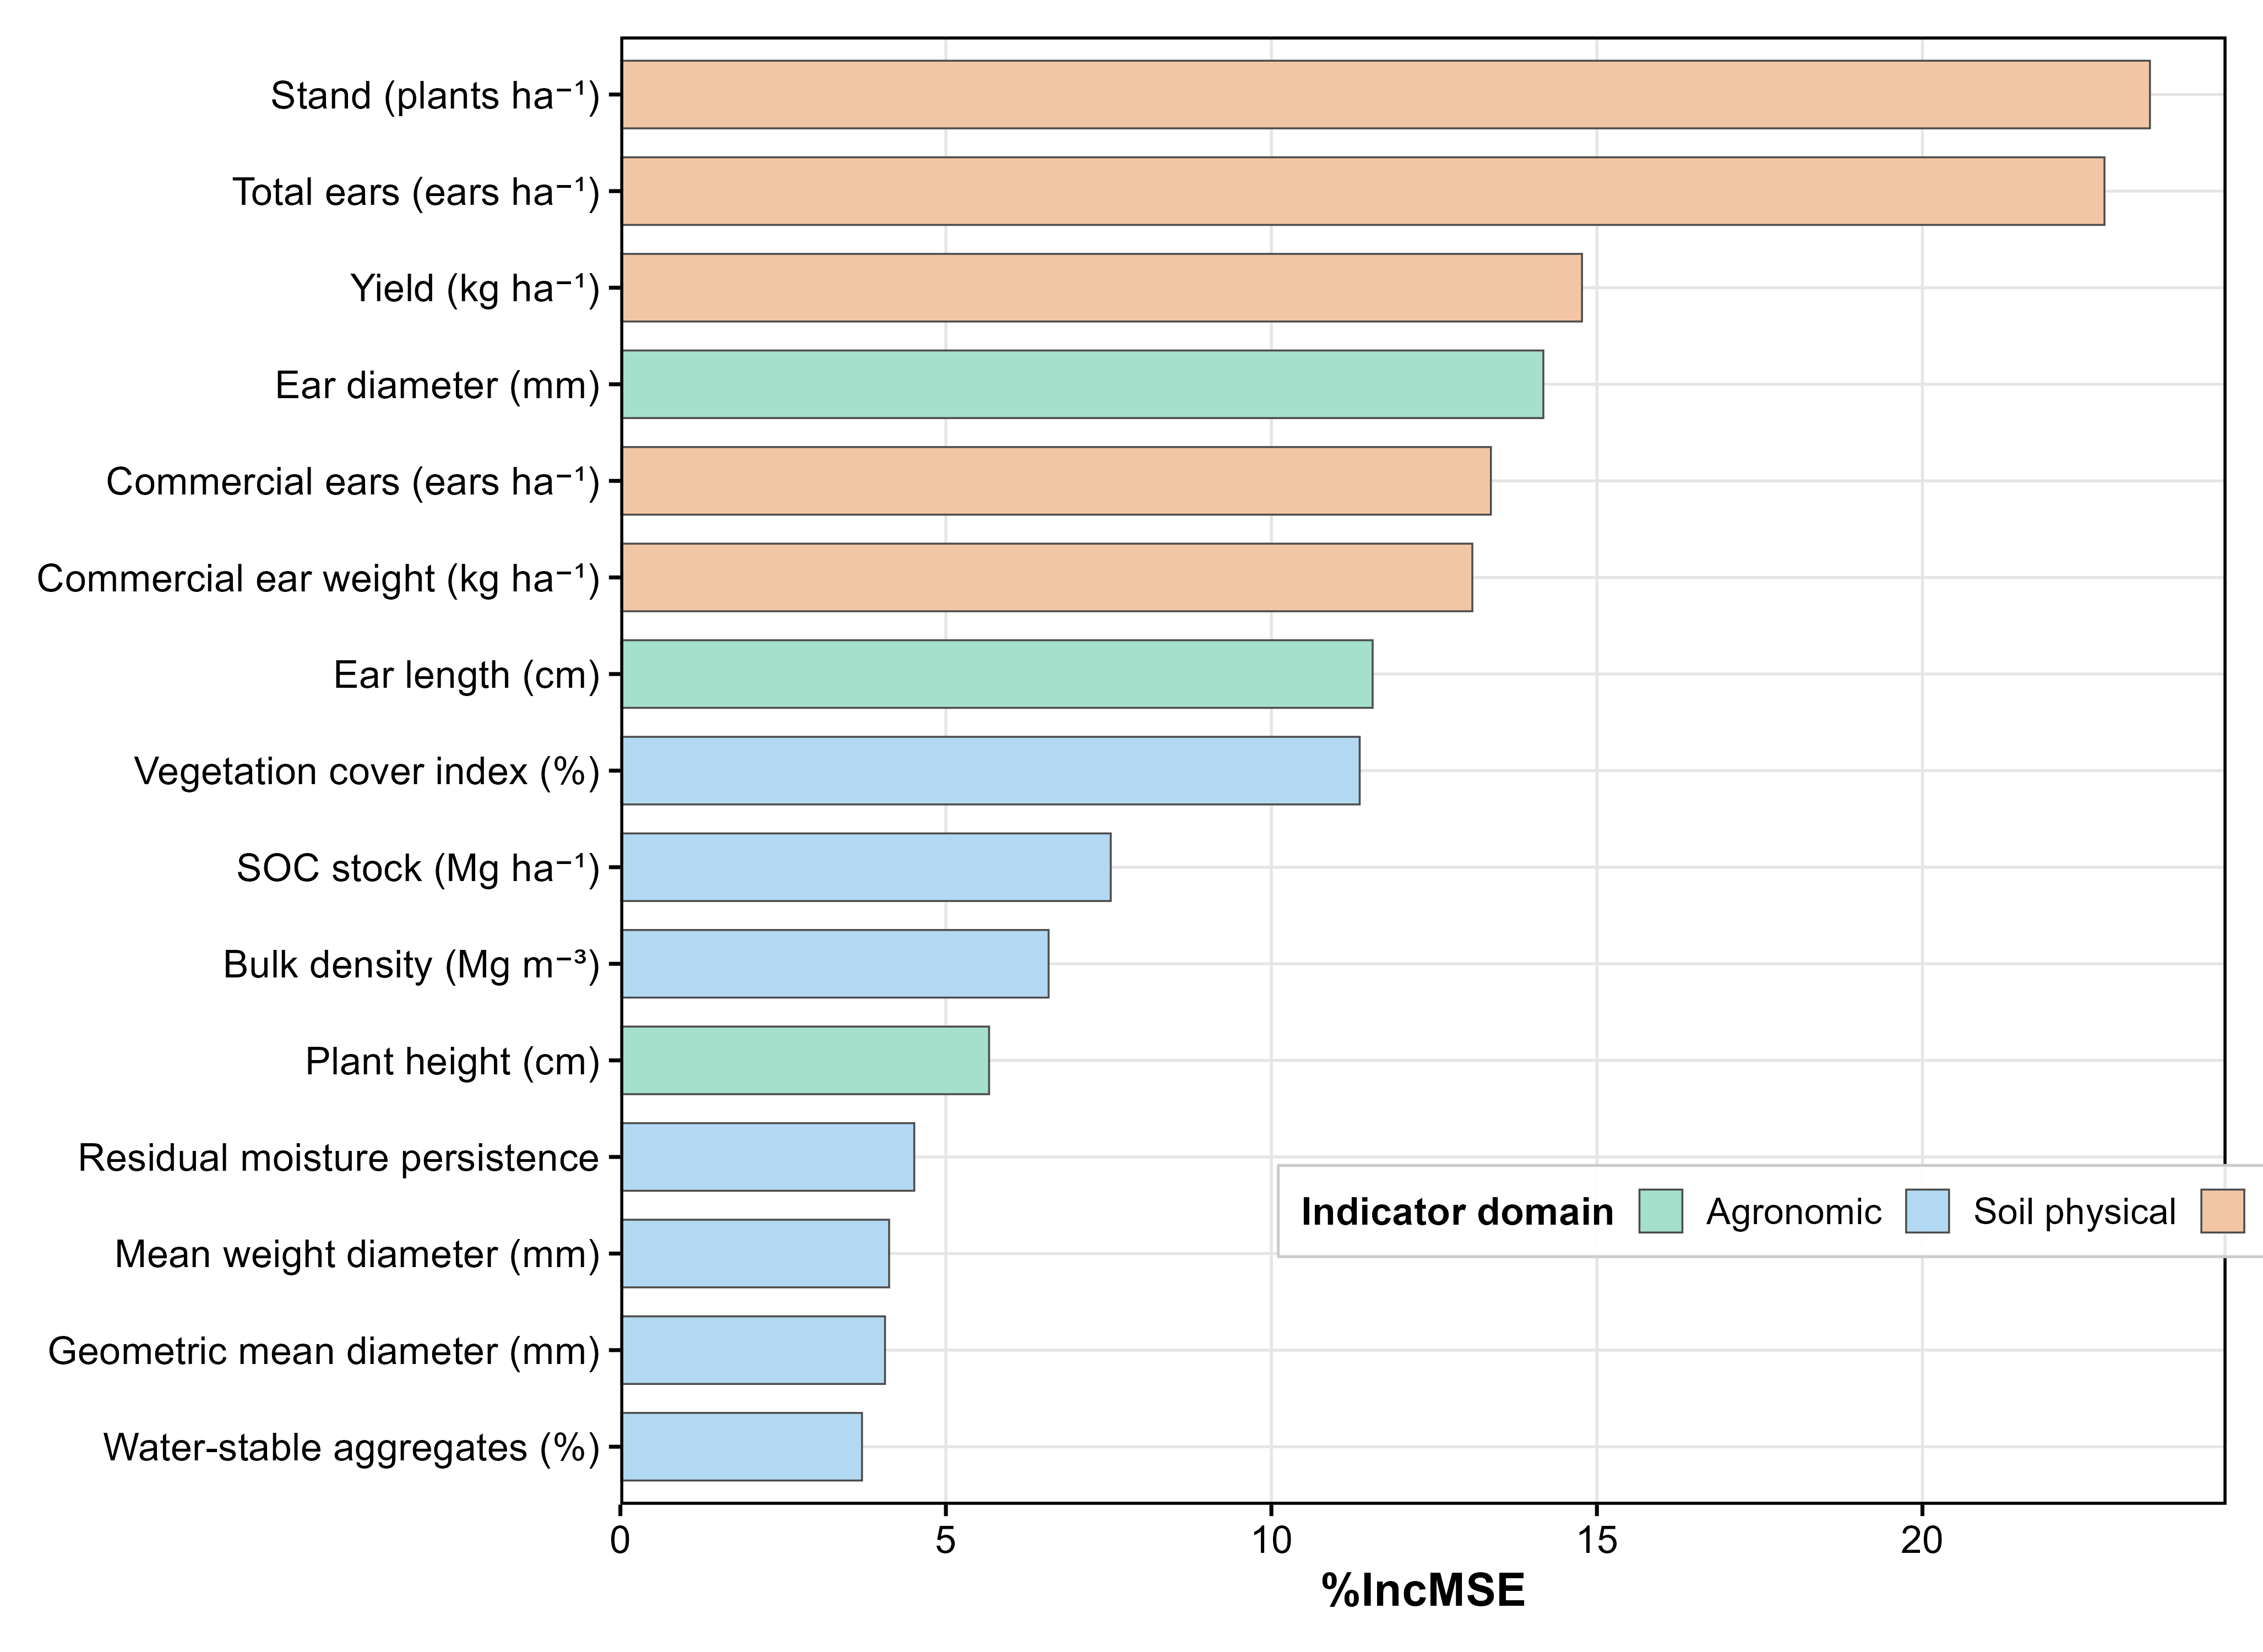
\includegraphics[width=0.75\textwidth]{../../2-DADOS/3-FIGURAS/fig_rf_importance.png}
\caption{Importância das variáveis por permutação (\%IncMSE) no modelo RF.}\label{fig:importance}
\smallskip\noindent\textit{Nota:} Barras coloridas por domínio do indicador.
\end{figure}

As curvas de dependência parcial (Fig.~\ref{fig:pdp}) revelam que o número total de espigas por hectare e o número de plantas exibem resposta sigmoidal sobre o IQS predito pelo RF, com limiar de transição entre os valores normalizados 4 e 6, a partir do qual o efeito marginal se estabiliza em patamar assintótico. O diâmetro da espiga e a produtividade, por sua vez, apresentam resposta monotônica crescente com menor intensidade de saturação, sugerindo contribuição quasi-linear para o escore integrado \cite{Friedman2001}. Esse padrão de limiares pode refletir o efeito de compensação entre espécies de cobertura sob Argissolo com camada coesa, em que ganhos de produtividade se estabilizam a partir de determinado nível de estande, enquanto atributos morfológicos mantêm relação de dose-resposta gradual \cite{Assuncao2023}. \cite{Moitinho2020}, ao avaliarem fungos micorrízicos arbusculares sob plantio direto com rotação de milho/cobertura em Argissolo Vermelho, observaram que feijão-guandu e crotalária promoveram maior abundância de esporos e índice de estabilidade de agregados do que gramíneas em monocultura, sugerindo que a mediação biológica da rizosfera pode contribuir para o acoplamento entre qualidade física e resposta produtiva captado pelas PDPs.

\begin{figure}[ht]
\centering
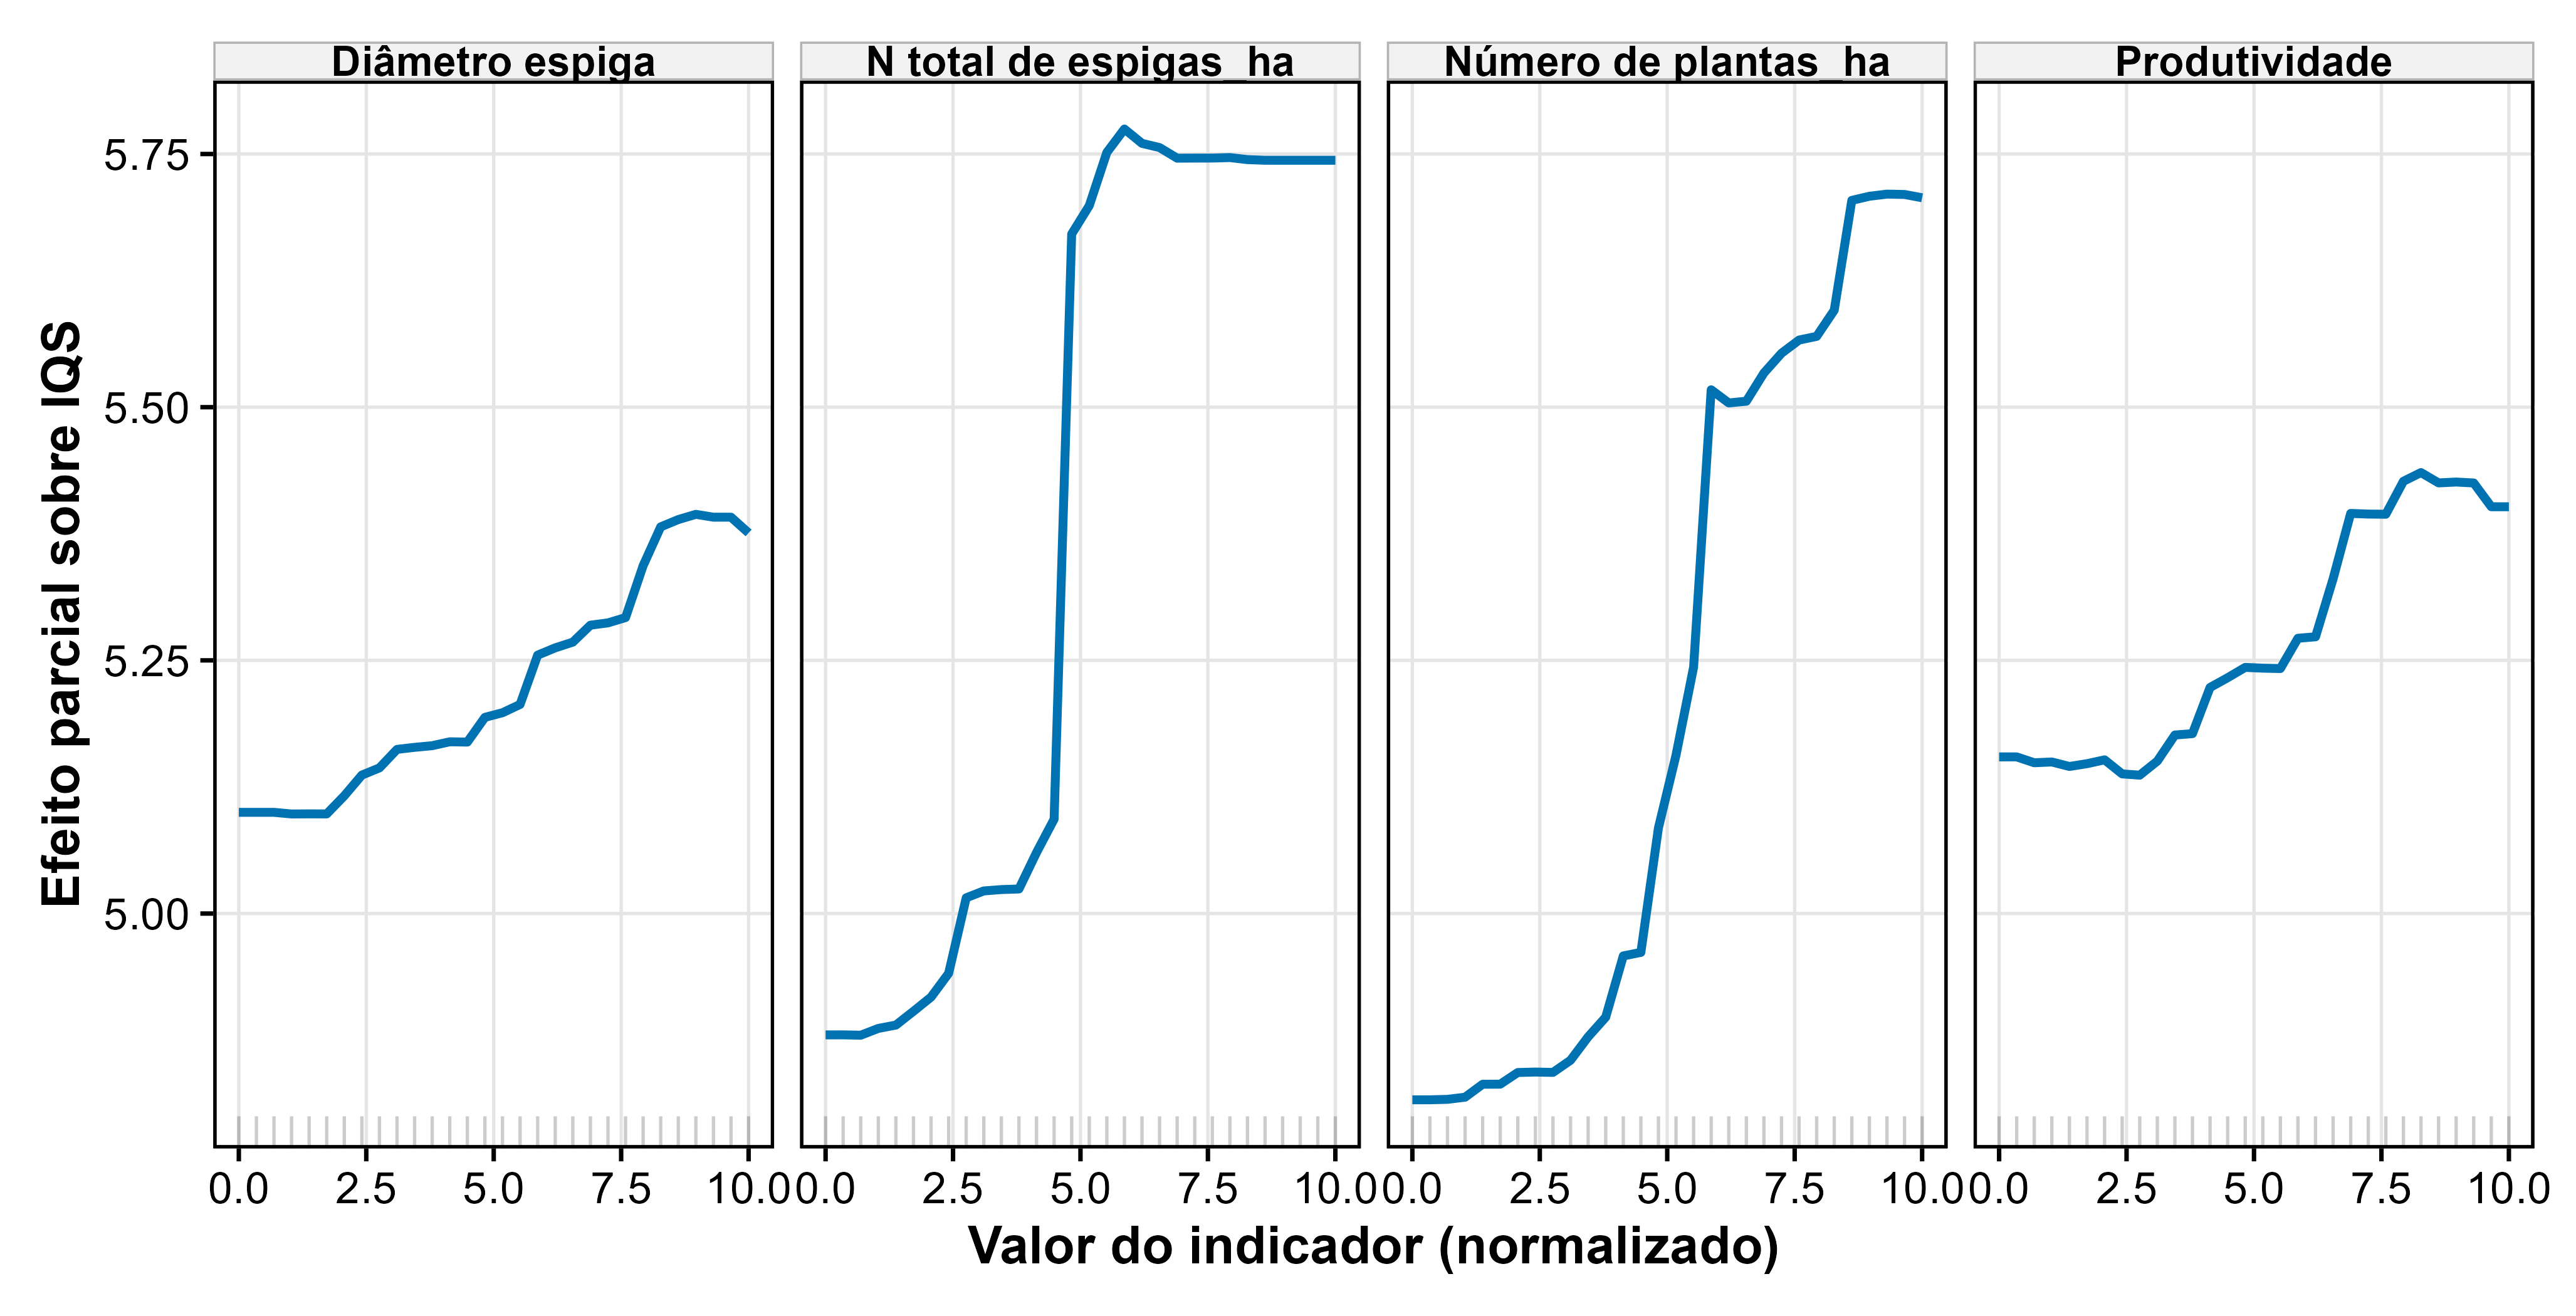
\includegraphics[width=\textwidth]{../../2-DADOS/3-FIGURAS/fig_pdp_top4.png}
\caption{Curvas de dependência parcial para os quatro indicadores de maior importância no modelo RF.}\label{fig:pdp}
\smallskip\noindent\textit{Nota:} Eixo horizontal, valor normalizado (0--10); eixo vertical, efeito parcial sobre o IQS predito. \textit{Rug plots} indicam a distribuição marginal dos dados.
\end{figure}

No modelo PLS-SEM, o construto AGRO explicou a maior parte da variância de REND ($\gamma = 0{,}803$, $p < 0{,}001$, IC\,95\% bootstrap: 0,699--0,896), ao passo que o caminho FISICO$\to$REND não atingiu significância ($\gamma = -0{,}052$, $p = 0{,}672$). Quatro indicadores foram excluídos do modelo estrutural por multicolinearidade (VIF\,$> 5$), o que pode subestimar a contribuição do domínio físico para o IQS latente. O construto de segunda ordem, obtido pelo primeiro componente principal dos três escores latentes, capturou 65,2\% da variância total, com carregamentos de 0,39 (FISICO), 0,66 (AGRO) e 0,64 (REND). Esse resultado é consistente com a mediação exercida pelo desempenho agronômico na relação solo--rendimento, padrão descrito em experimentos de longa duração sobre Argissolos com camada coesa \cite{Nabiollahi2018}. O peso desproporcional do construto AGRO pode refletir a contribuição da fixação biológica de nitrogênio (FBN) ao sistema. \cite{Berriel2023}, em estudo conduzido no Uruguai, quantificaram a FBN de \textit{Cajanus cajan} em 120--180~kg~N~ha$^{-1}$~ano$^{-1}$ quando utilizado como cobertura, valor entre três e seis vezes superior ao de gramíneas forrageiras temperadas. Em sistemas tropicais de longa duração como o presente, o aporte cumulativo de N pode condicionar o desempenho agronômico de forma que ultrapassa a variabilidade explicável pelos indicadores físicos na camada superficial.

Os cinco paradigmas produziram distribuições de IQS com amplitude e dispersão distintas. SIF, MARS e RF apresentaram médias próximas (5,24 na escala 0--10), enquanto o IQS$_{\text{PLS}}$ (média\,$=$\,4,18) e o IQS$_{\text{ANOVA}}$ (média\,$=$\,4,39) ocuparam faixas mais amplas (0--10), reflexo da linearidade e da redução dimensional impostas por esses paradigmas.

\subsection{Concordância inter-paradigma e meta-IQS}\label{subsec:concordance_disc}

O coeficiente de concordância de Kendall ($W = 0{,}808$, $\chi^2 = 432{,}0$, $p < 2{,}2 \times 10^{-16}$) sustentou $H_1$ \cite{Legendre2012}, indicando concordância significativa entre os cinco ranqueamentos simultâneos. O teste de permutação (10\,000 repetições) corroborou esse resultado ($p < 0{,}0001$). O ICC(2,1) de 0,721 (IC\,95\%: 0,654--0,783) indica concordância absoluta substancial, embora inferior ao limiar de 0,75 geralmente considerado ``bom'' em aplicações de confiabilidade \cite{Koo2016}. O coeficiente AC1 de Gwet, calculado sobre quintis dos valores de IQS, foi de 0,402, valor mais conservador que reflete a penalização por concordância marginal esperada ao acaso.

A matriz de correlação de Spearman revelou uma estrutura de três camadas (Tabela~\ref{tab:spearman}). SIF, MARS e RF formaram um bloco quase indistinguível ($\rho > 0{,}993$ entre quaisquer pares, correspondendo a 30\% das comparações par a par), o PLS-SEM ocupou posição intermediária ($\rho = 0{,}679$--$0{,}685$ com os três anteriores, 30\% das comparações) e o paradigma ANOVA divergiu de todos os demais ($\rho = 0{,}589$--$0{,}602$ com SIF, MARS e RF, 40\% das comparações), embora tenha apresentado correlação moderada com o PLS-SEM ($\rho = 0{,}782$). O teste de Wilcoxon sustentou $H_2$ ($W = 21$, $p = 0{,}033$), com média de $\rho$ entre pares não lineares ($\bar{\rho}_{\text{NL-NL}} = 0{,}838$) superior à observada entre pares linear--não linear ($\bar{\rho}_{\text{Lin-NL}} = 0{,}642$).

\begin{table}[ht]
\caption{Matriz de correlação de Spearman ($\rho$) entre os cinco paradigmas de IQS após transformação de Blom.}\label{tab:spearman}
\begin{tabular*}{\textwidth}{@{\extracolsep\fill}lccccc}
\toprule
 & ANOVA & Fuzzy & PLS-SEM & MARS & RF \\
\midrule
ANOVA   & 1,000 & 0,593 & 0,782 & 0,589 & 0,602 \\
Fuzzy   &       & 1,000 & 0,679 & 0,995 & 0,995 \\
PLS-SEM &       &       & 1,000 & 0,681 & 0,685 \\
MARS    &       &       &       & 1,000 & 0,993 \\
RF      &       &       &       &       & 1,000 \\
\botrule
\end{tabular*}
\end{table}

A representação gráfica dessa matriz por heatmap anotado (Fig.~\ref{fig:heatmap}) permite identificar visualmente o agrupamento em blocos de concordância.

\begin{figure}[ht]
\centering
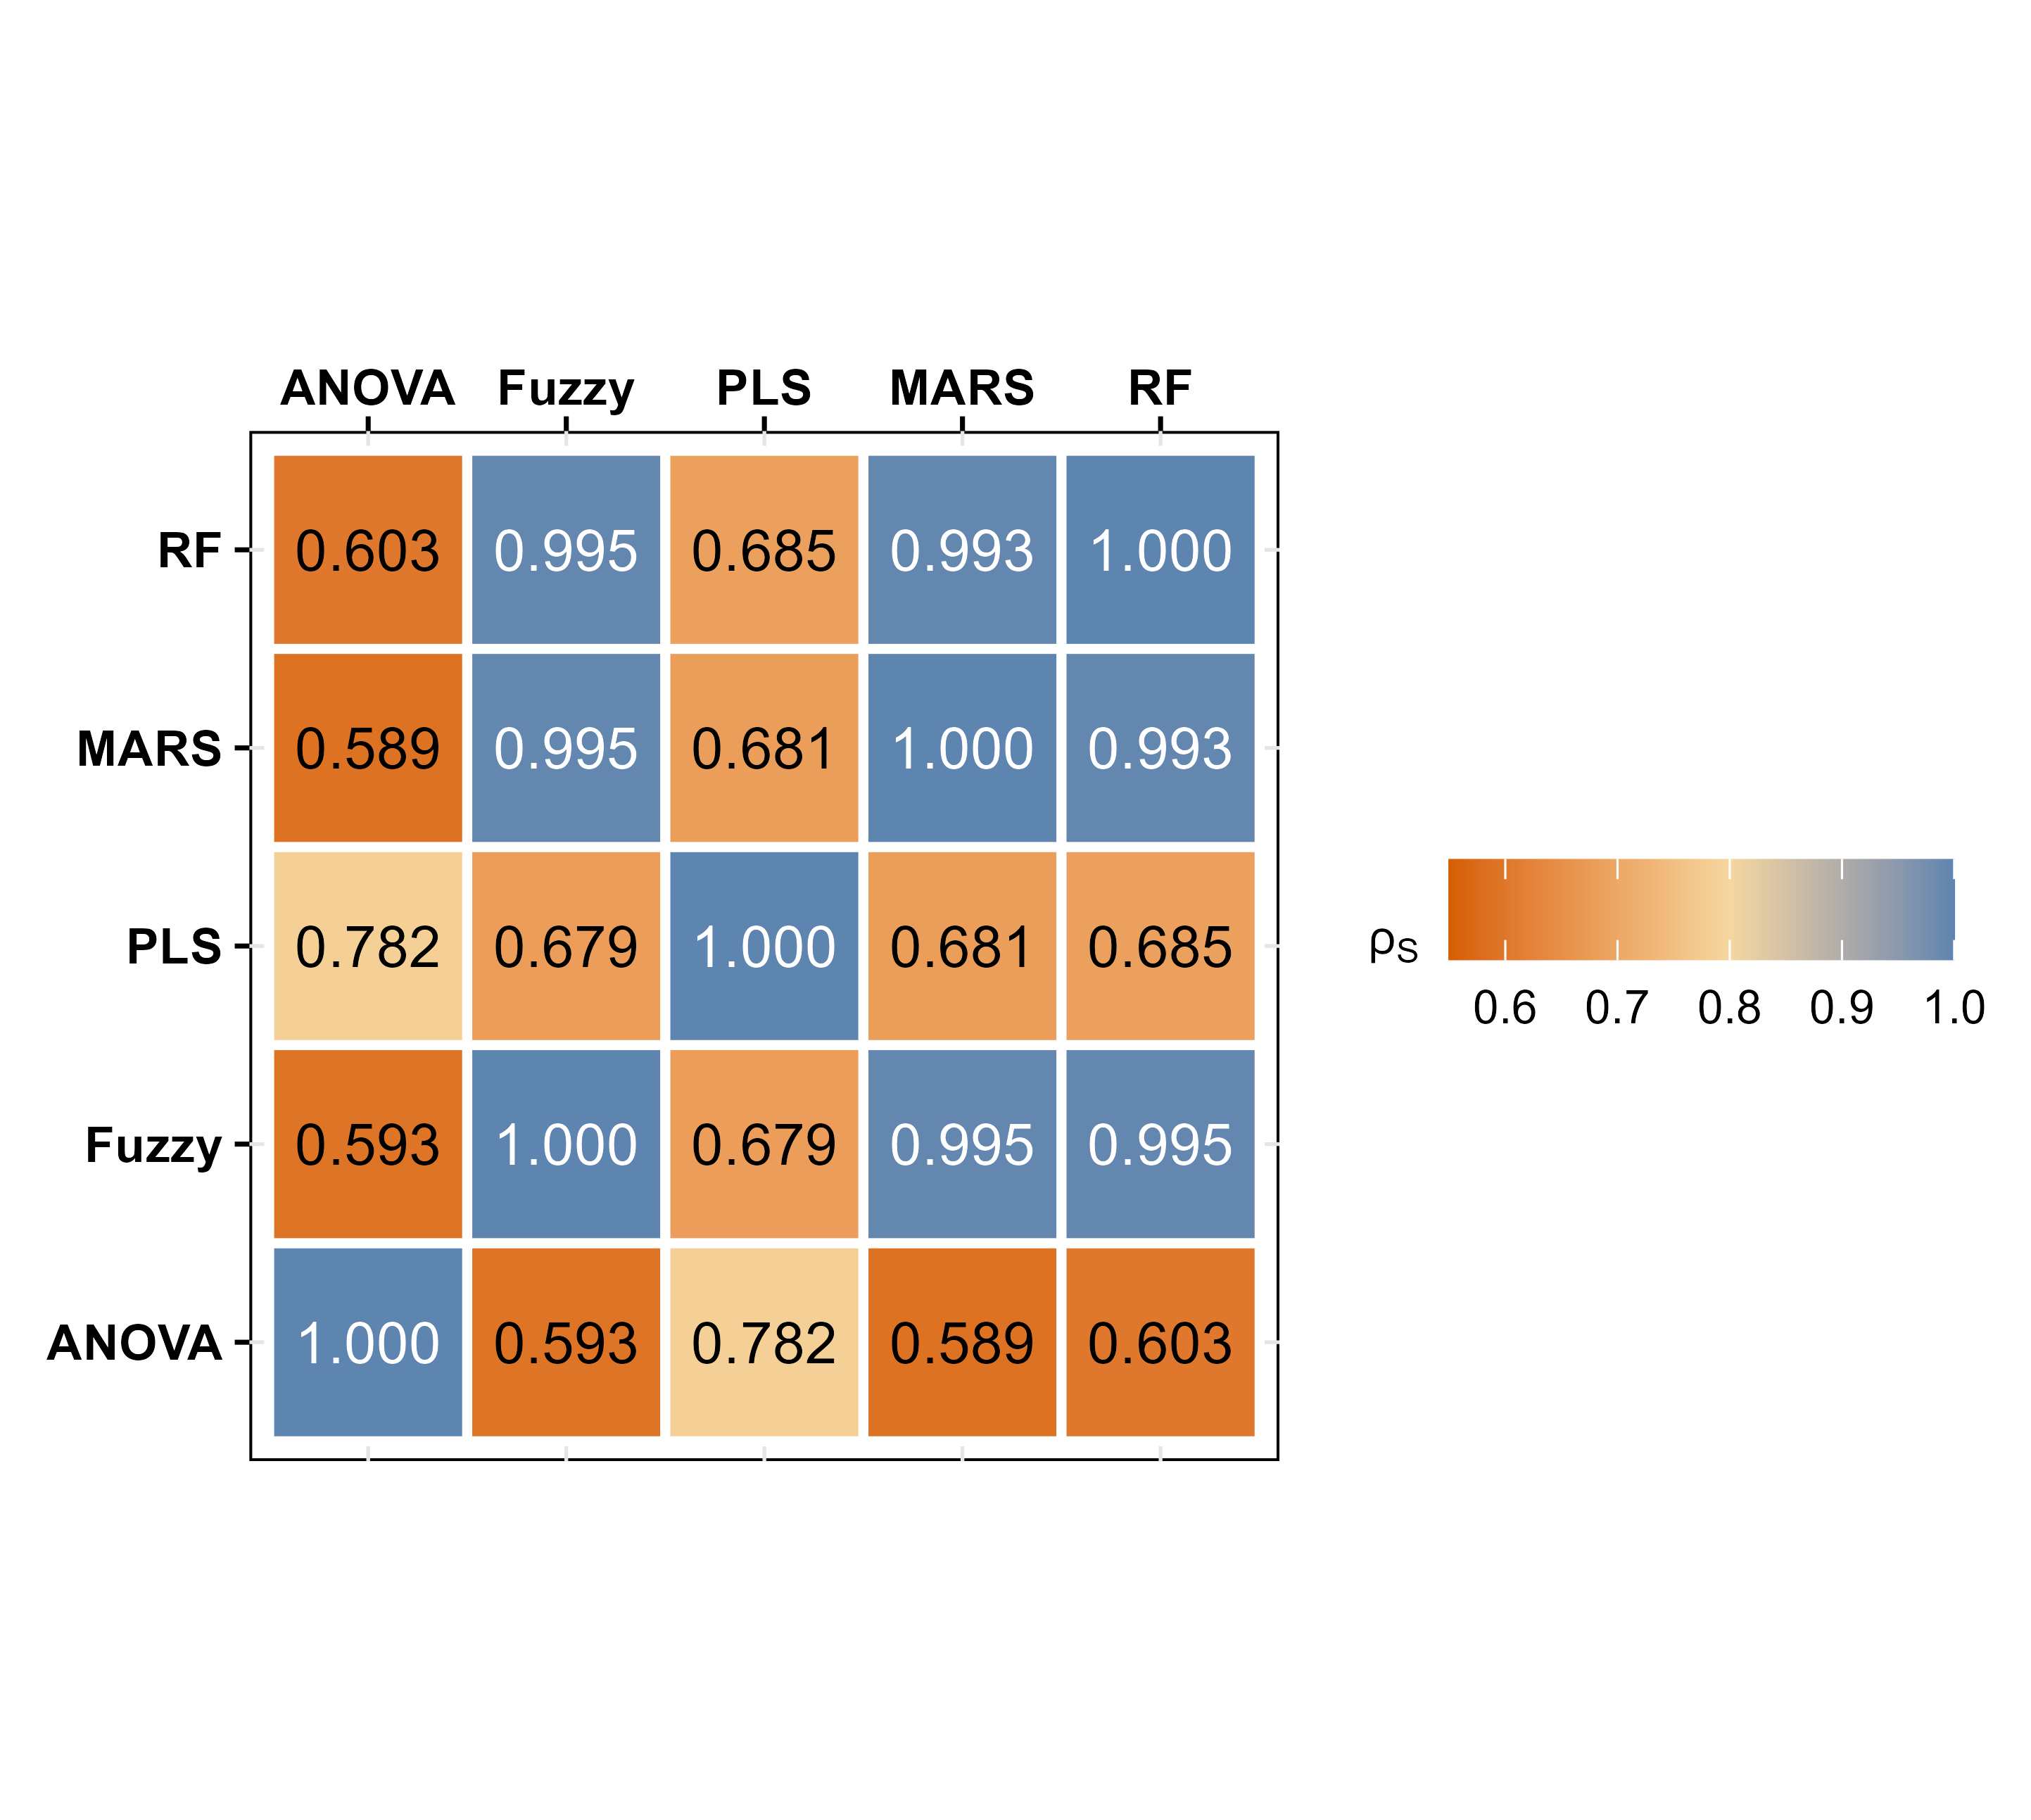
\includegraphics[width=0.55\textwidth]{../../2-DADOS/3-FIGURAS/fig_heatmap_spearman.png}
\caption{Heatmap da matriz de correlação de Spearman ($\rho_S$) entre os cinco paradigmas de IQS (escala Blom).}\label{fig:heatmap}
\smallskip\noindent\textit{Nota:} Valores anotados em cada célula. Escala de cor de laranja ($\rho \approx 0{,}59$) a azul ($\rho = 1{,}00$).
\end{figure}

O gradiente de cor separa o bloco SIF-MARS-RF (tons frios, $\rho > 0{,}99$) dos pares envolvendo ANOVA (tons quentes, $\rho < 0{,}60$), ao passo que o PLS-SEM ocupa faixa cromática intermediária ($\rho \approx 0{,}68$ com o bloco não linear), reforçando sua posição de transição entre os dois agrupamentos. Para quantificar a magnitude prática dessa separação em termos de intercambialidade entre paradigmas, os limites de concordância obtidos pela análise de Bland--Altman \cite{BlandAltman1986} (Tabela~\ref{tab:blandaltman}) reforçaram quantitativamente essa estrutura tricamada. Os LoA entre pares do bloco SIF-MARS-RF variaram de $\pm 0{,}33$ (Fuzzy vs.\ RF) a $\pm 0{,}50$ (MARS vs.\ RF) na escala Blom, sugerindo substituibilidade prática em 30\% das comparações. Em contraste, os pares envolvendo o PLS-SEM apresentaram LoA intermediários ($\pm 1{,}63$--$1{,}68$, 30\% das comparações), e os pares com ANOVA exibiram LoA de até $\pm 1{,}93$ (40\% das comparações), indicando que a substituição do paradigma linear por qualquer alternativa não linear pode alterar posições de ranqueamento individuais.

\begin{table}[ht]
\caption{Sumário da análise de Bland--Altman entre pares de paradigmas (escala Blom).}\label{tab:blandaltman}
\begin{tabular*}{\textwidth}{@{\extracolsep\fill}lcccc}
\toprule
Par & $\bar{d}$ & $s_d$ & LoA inf. & LoA sup. \\
\midrule
Fuzzy vs RF    & 0,00 & 0,170 & $-$0,332 & 0,332 \\
Fuzzy vs MARS  & 0,00 & 0,225 & $-$0,440 & 0,441 \\
MARS vs RF     & 0,00 & 0,256 & $-$0,503 & 0,502 \\
PLS vs Fuzzy   & 0,00 & 0,847 & $-$1,661 & 1,661 \\
PLS vs MARS    & 0,00 & 0,856 & $-$1,677 & 1,677 \\
PLS vs RF      & 0,00 & 0,831 & $-$1,629 & 1,629 \\
ANOVA vs PLS   & 0,00 & 0,724 & $-$1,420 & 1,420 \\
ANOVA vs Fuzzy & 0,00 & 0,967 & $-$1,896 & 1,896 \\
ANOVA vs MARS  & 0,00 & 0,982 & $-$1,924 & 1,925 \\
ANOVA vs RF    & 0,00 & 0,946 & $-$1,854 & 1,854 \\
\botrule
\end{tabular*}
\smallskip\noindent\textit{Nota:} $\bar{d}$, diferença média; $s_d$, desvio-padrão da diferença; LoA, limites de concordância ($\pm 1{,}96\,s_d$).
\end{table}

Três pares representativos, um de cada camada de concordância, foram selecionados para representação gráfica dos limites de Bland--Altman (Fig.~\ref{fig:ba_panel}).

\begin{figure}[ht]
\centering
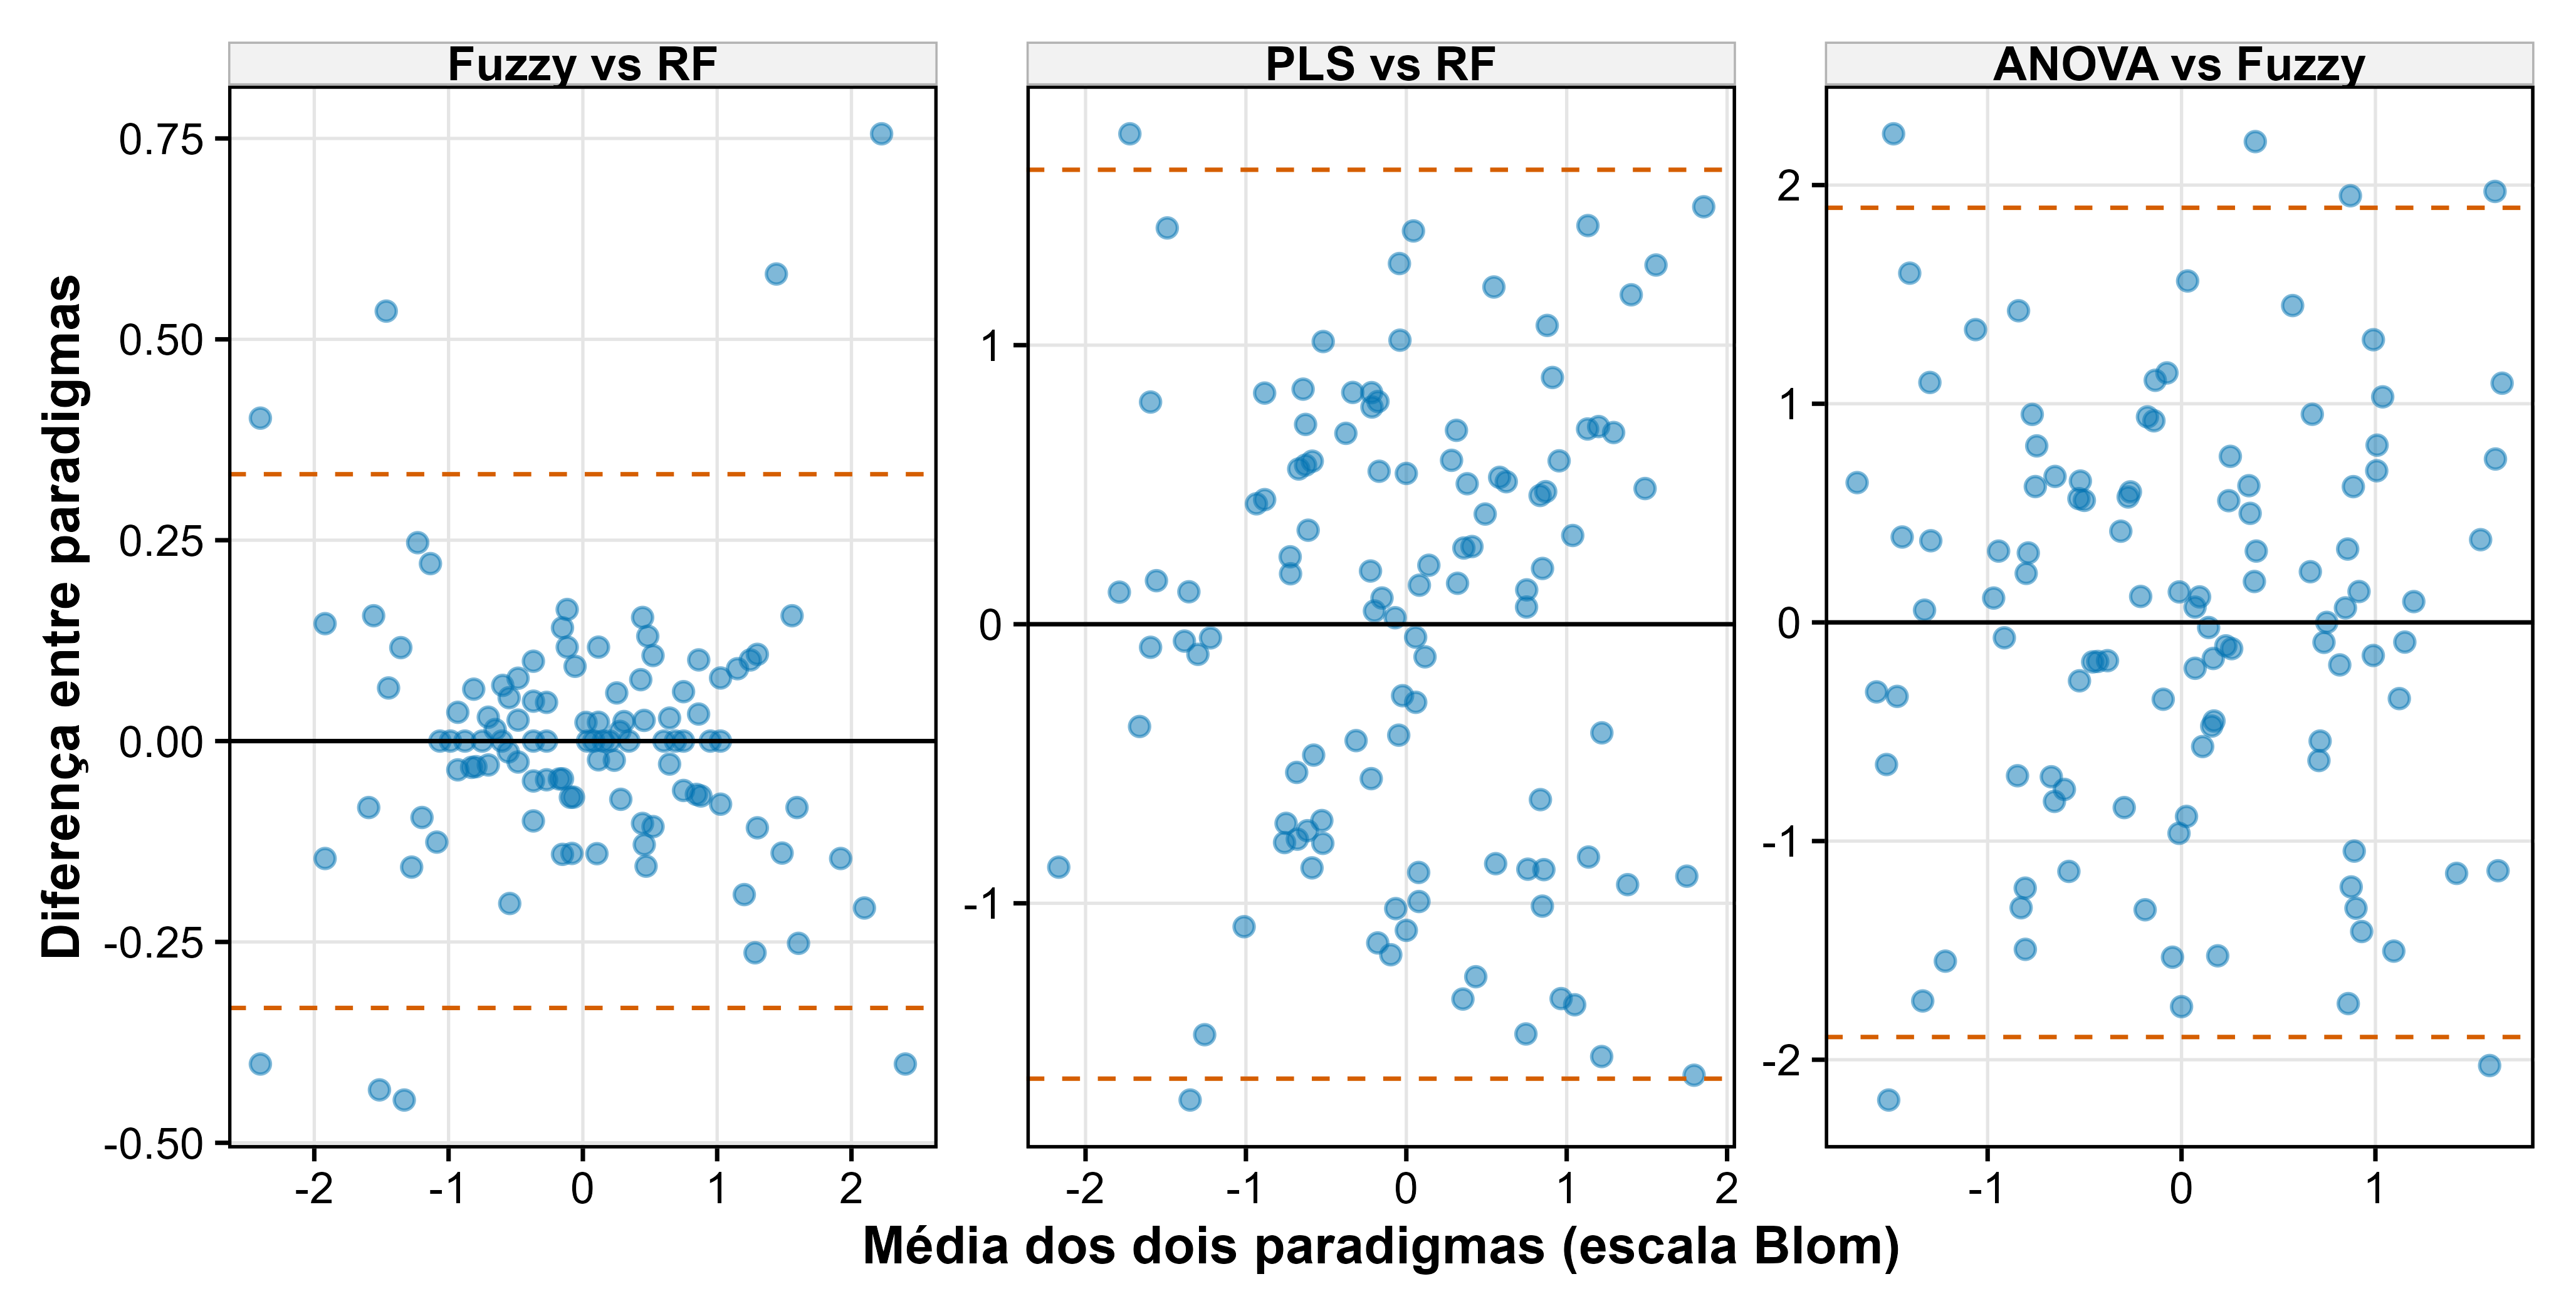
\includegraphics[width=\textwidth]{../../2-DADOS/3-FIGURAS/fig_blandaltman_panel.png}
\caption{Diagramas de Bland--Altman para três pares representativos de paradigmas (escala Blom).}\label{fig:ba_panel}
\smallskip\noindent\textit{Nota:} Linha contínua, diferença média ($\bar{d} \approx 0$); linhas tracejadas, limites de concordância a $\pm 1{,}96\,s_d$.
\end{figure}

O par Fuzzy--RF exibe pontos concentrados na faixa $\pm 0{,}33$ com dispersão homogênea ao longo do eixo de médias, confirmando substituibilidade prática dentro do bloco não linear. O par ANOVA--Fuzzy, em contraste, apresenta padrão em leque que sugere viés proporcional ao nível do IQS \cite{Giavarina2015}, ao passo que o par PLS--RF ocupa posição intermediária (LoA\,$\approx \pm 1{,}63$), com aparente heteroscedasticidade nos valores extremos, indicando que a discordância é mais acentuada para combinações de manejo com qualidade inferior. Embora os diagramas de Bland--Altman quantifiquem a concordância absoluta, a variância compartilhada entre paradigmas pode ser avaliada por diagramas de dispersão 1:1, com o RF adotado como referência (Fig.~\ref{fig:scatter1to1}).

\begin{figure}[ht]
\centering
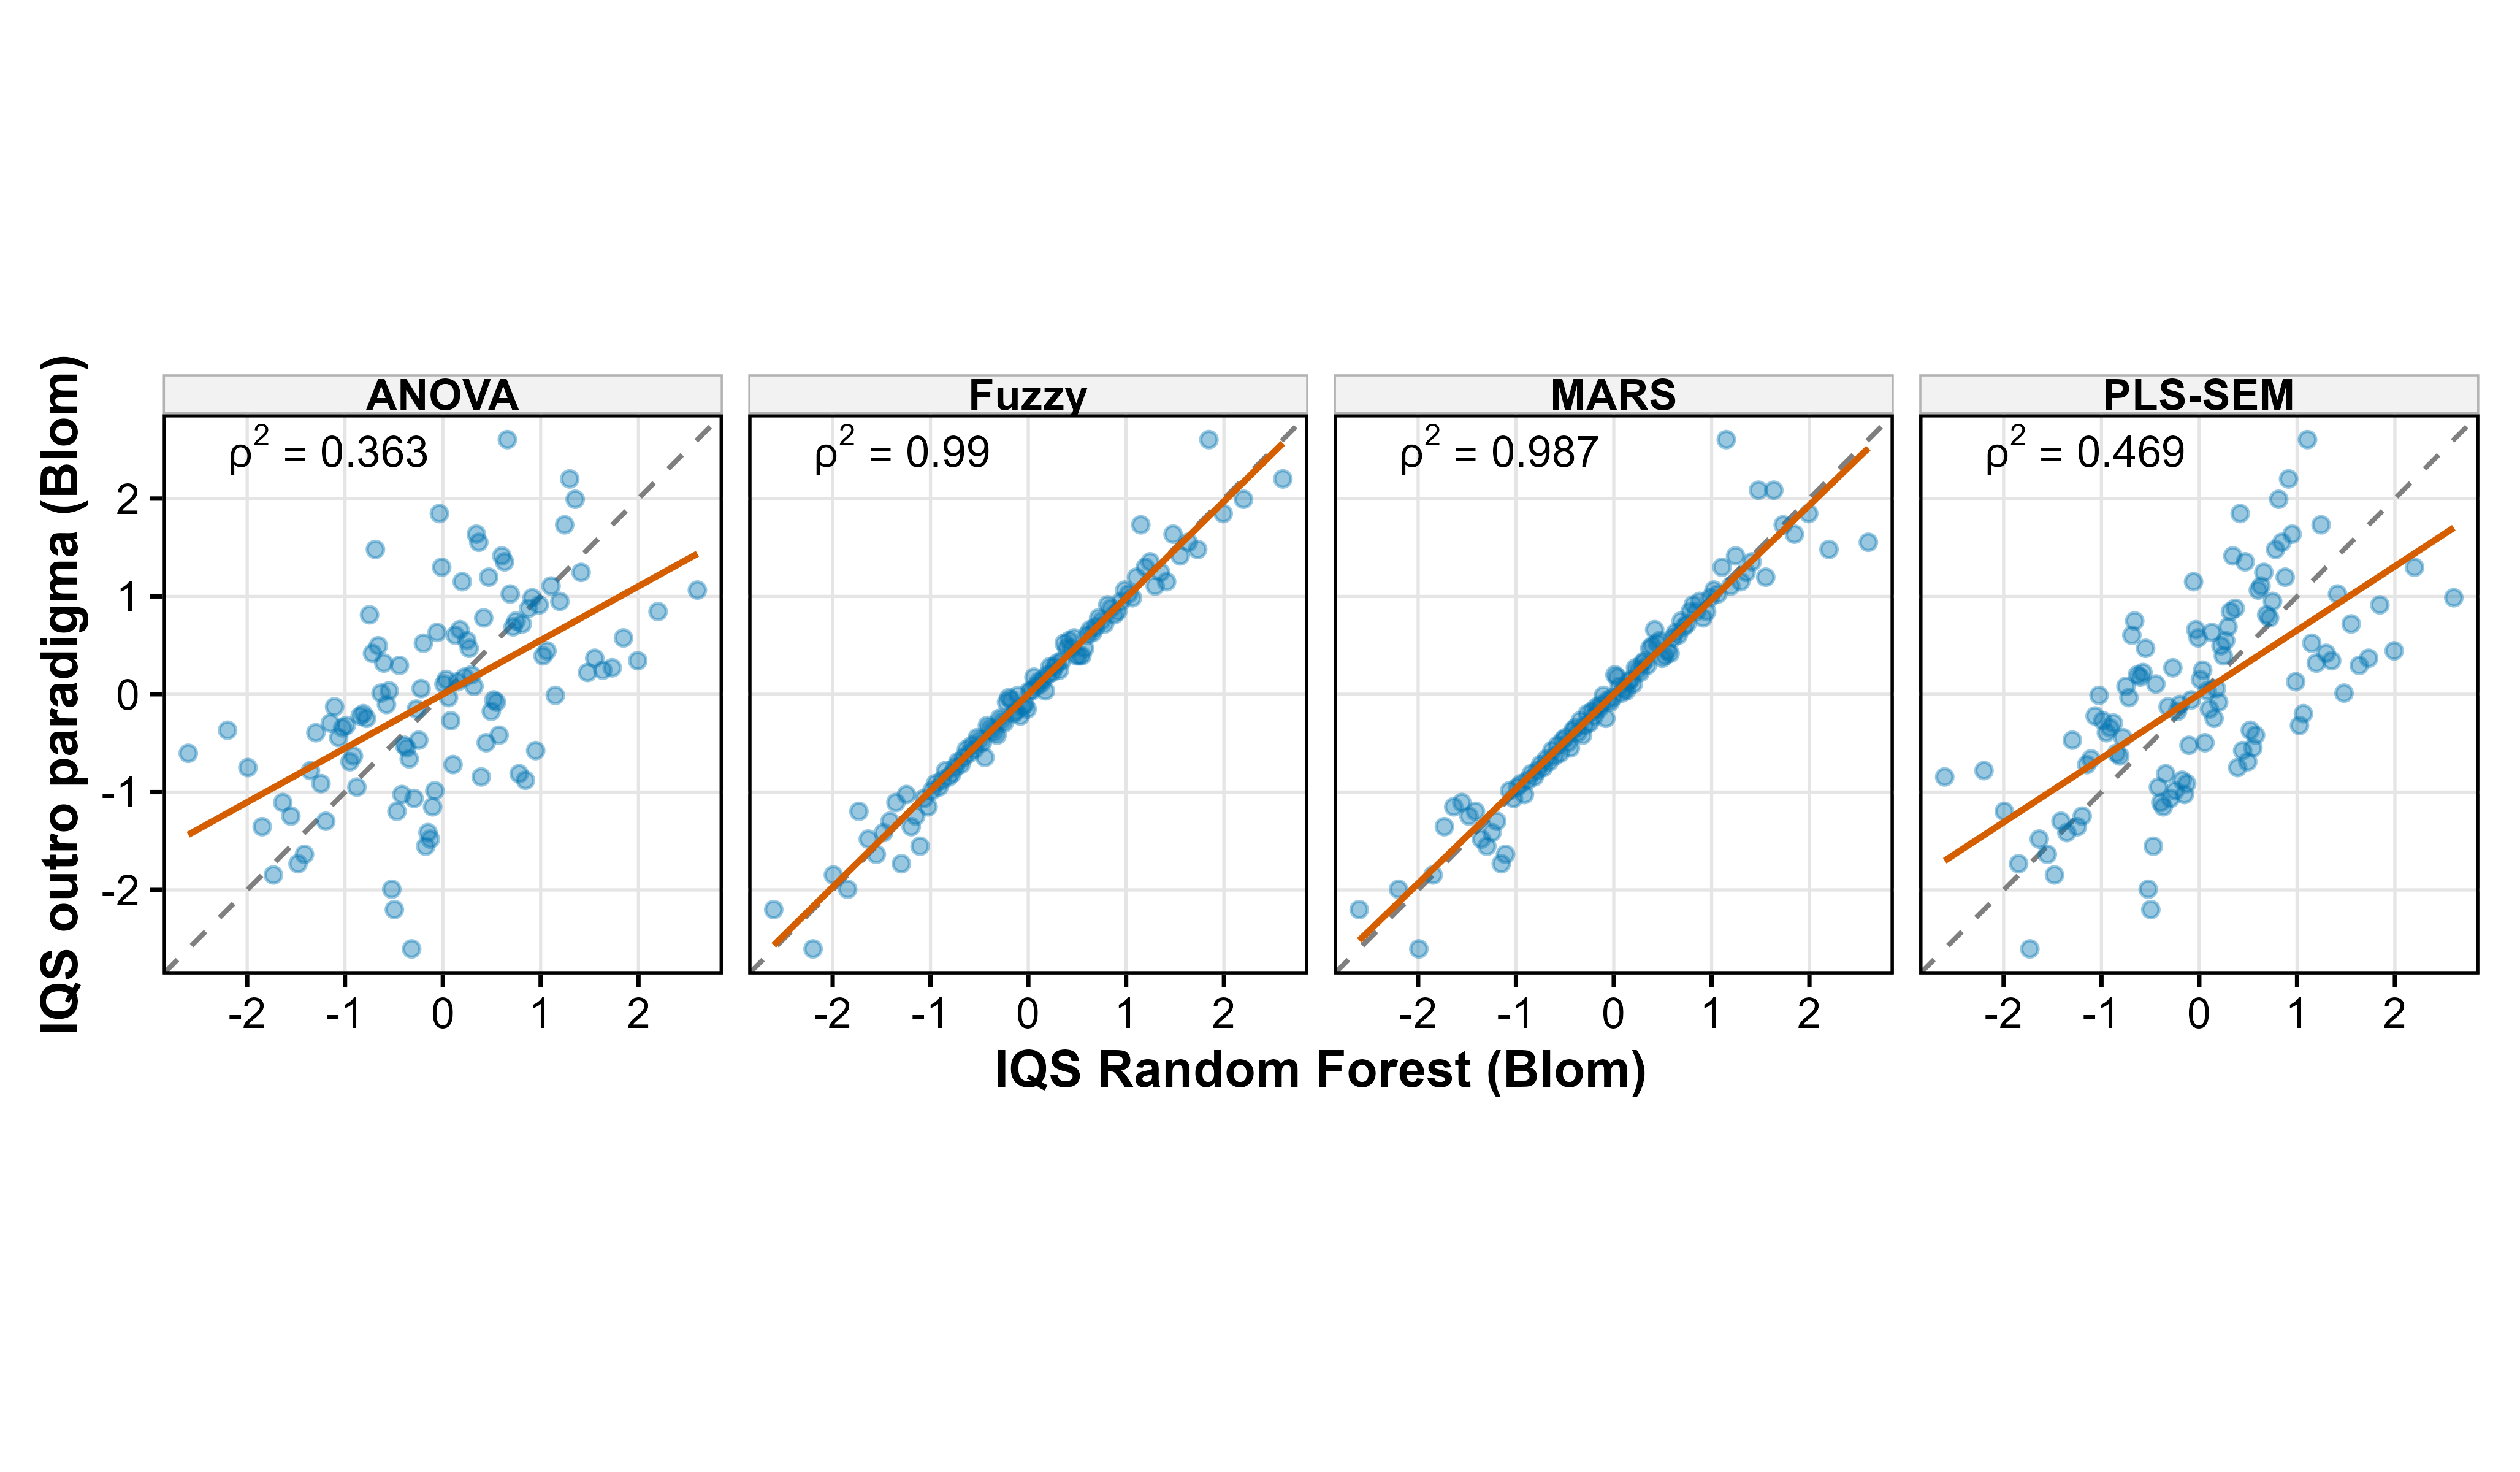
\includegraphics[width=\textwidth]{../../2-DADOS/3-FIGURAS/fig_scatter_1to1.png}
\caption{Diagramas de dispersão 1:1 de IQS (escala Blom) entre cada paradigma e o RF como referência.}\label{fig:scatter1to1}
\smallskip\noindent\textit{Nota:} Linha tracejada, identidade; linha contínua, regressão local. Valores de $\rho^2$ anotados em cada painel.
\end{figure}

Fuzzy ($\rho^2 = 0{,}990$) e MARS ($\rho^2 = 0{,}987$) alinham-se quase perfeitamente com a diagonal de identidade, ao passo que ANOVA ($\rho^2 = 0{,}363$) e PLS-SEM ($\rho^2 = 0{,}469$) apresentam dispersão pronunciada, com observações individuais desviando em até 1,5 unidades Blom da reta 1:1 \cite{Venkateswarlu2025}. 

Essa magnitude de desvio implica que, para uma dada observação, o diagnóstico de qualidade ``alta'' ou ``baixa'' pode ser contingente ao paradigma quando se adota o limiar convencional da mediana, padrão que reforça a necessidade de métricas de concordância na avaliação de IQS \cite{Liu2025}. \cite{Kahsay2025}, ao compararem oito modelos de IQS (TDS/MDS $\times$ escore linear/não linear $\times$ IQI/NQI) em terras degradadas da Etiópia, verificaram que a função de escore não linear produziu índices sistematicamente 12--18\% superiores ao escore linear, com divergência amplificada em solos de baixa qualidade. 

Esse padrão é consistente com o viés em leque observado no diagrama de Bland--Altman do par ANOVA--Fuzzy (Fig.~\ref{fig:ba_panel}), onde a discordância cresce com o nível do IQS, sugerindo que a compressão linear subestima a qualidade em solos de baixo desempenho. \cite{Zhang2024LDD}, em rotação trigo--milho sob plantio convencional e conservacionista no norte da China, reportaram que o IQS com escore não linear detectou benefícios do manejo conservacionista que o escore linear não distinguiu, o que reforça a hipótese de que a família analítica, e não apenas o conjunto de indicadores, condiciona a sensibilidade do índice.

A convergência entre SIF, MARS e RF é consistente com a hipótese de que esses paradigmas acessam o mesmo subespaço de variabilidade, definido por relações não lineares e interações de alta ordem entre indicadores que o modelo linear comprime ou ignora \cite{Zeraatpisheh2020,Wadoux2020}. \cite{DosSantos2021} observaram padrão análogo em Latossolo Vermelho sob sistemas integrados de produção, com o IQS fuzzy detectando diferenças de manejo que o protocolo aditivo clássico não distinguiu, o que sustenta a generalidade da convergência não linear em solos tropicais. 

Em analise comparativa de modelos SQI$_w$ e SQI$_c$ em seis classes de uso da terra no Irã central \cite{Emami2024}, reportaram divergência de até 30\% entre índices aditivos ponderados e índices cumulativos em solos com distribuição heterogênea de indicadores, o que é consistente com a amplitude dos LoA observados neste estudo para pares envolvendo a ANOVA.  \cite{Mahajan2021}, ao compararem três métodos de indexação (SQI$_w$ aditivo, SQI$_n$ Nemoro e SQI$_c$ cumulativo) em solos costeiros salinos da Índia, observaram que a concordância entre métodos variava com a severidade da salinidade, sendo mais elevada em solos com qualidade intermediária e menor nos extremos, padrão que se assemelha à heteroscedasticidade dos diagramas de Bland--Altman aqui reportados. 

O PLS-SEM, por especificar caminhos lineares entre construtos latentes mas incorporar indicadores formativos (Mode~B) que capturam parcialmente a não linearidade na composição \cite{Diamantopoulos2008}, ocupa posição intermediária, com LoA de $\pm 1{,}65$ que são da mesma magnitude da variabilidade entre-parcelas reportada por \cite{Oliveira2020} para Argissolos sob plantio direto de longa duração no Nordeste brasileiro. A divergência da ANOVA é consistente com a dependência de pesos derivados de ACP e de combinação linear de escores ortogonais, que perdem informação sobre interações de ordem superior \cite{Andrews2002,Bünemann2018}, indicando que a substituibilidade entre paradigmas depende da família analítica, e não do algoritmo específico.

\cite{Mukherjee2014} observaram diferenças absolutas de até 15\% entre três variantes de escorificação (aditiva, ponderada e média geométrica), embora a ordenação relativa dos usos tenha sido preservada, o que antecipou qualitativamente a convergência de extremos aqui quantificada ($W = 0{,}81$, ICC\,=\,0{,}72). \cite{Chaudhry2024} reportaram convergência moderada entre modelos estatísticos e de AM, porém restringiram a comparação a paradigmas da mesma família, sem inferência fuzzy ou equações estruturais. \cite{Pacci2026} integraram lógica fuzzy hesitante com AHP e inteligência artificial com ganho de resolução, mas limitaram a análise a um único tipo de solo sem métrica de concordância inter-avaliador. A confrontação simultânea de cinco famílias com pressupostos estruturalmente distintos, associada a protocolo formal de concordância ($W$, ICC, Bland--Altman), permitiu quantificar limiares de substituibilidade ($\rho > 0{,}99$ e LoA\,$< \pm 0{,}50$ para o bloco SIF-MARS-RF) que podem servir como referência em futuros exercícios de benchmarking de IQS.

O meta-IQS obtido por contagem de Borda apresentou correlação de Spearman $\geq 0{,}95$ com SIF, MARS e RF, de 0,85 com PLS-SEM e de 0,79 com ANOVA, sugerindo que a agregação ordinal dos cinco paradigmas recupera o consenso do bloco não linear. Esses limiares de concordância constituem, até onde se pode verificar, a primeira referência quantitativa multi-família para substituibilidade de paradigmas de IQS em ensaios de campo. Pesquisadores que necessitem justificar a adoção de um paradigma específico podem apoiar-se nos valores aqui reportados como critérios operacionais de decisão. Pares de métodos com $\rho > 0{,}99$ e LoA\,$< \pm 0{,}50$ (30\% das comparações) são intercambiáveis para fins de ranqueamento de manejo, ao passo que pares com $\rho \approx 0{,}68$ e LoA\,$\approx \pm 1{,}65$ (30\% das comparações) podem produzir divergências em posições intermediárias sem alterar extremos. Pares com $\rho < 0{,}60$ e LoA\,$> \pm 1{,}85$ (40\% das comparações, todos envolvendo a ANOVA), podem inverter posições de manejo, exigindo verificação de sensibilidade antes de qualquer recomendação agronômica.

\subsection{Ranqueamento por combinação manejo--cobertura}\label{subsec:ranking}

A distribuição dos escores de IQS por combinação manejo--cobertura (Fig.~\ref{fig:boxplot_combo}) evidencia que o cultivo mínimo com feijão-guandu (CM-Guandu) concentrou os maiores valores medianos para todos os cinco paradigmas, com amplitudes interquartílicas reduzidas que sugerem baixa variabilidade interna nessa combinação. No extremo oposto, plantio convencional com feijão-guandu (PC-Guandu) exibiu os escores mais baixos em todos os paradigmas, com medianas próximas de 1,0 na escala original.

\begin{figure}[ht]
\centering
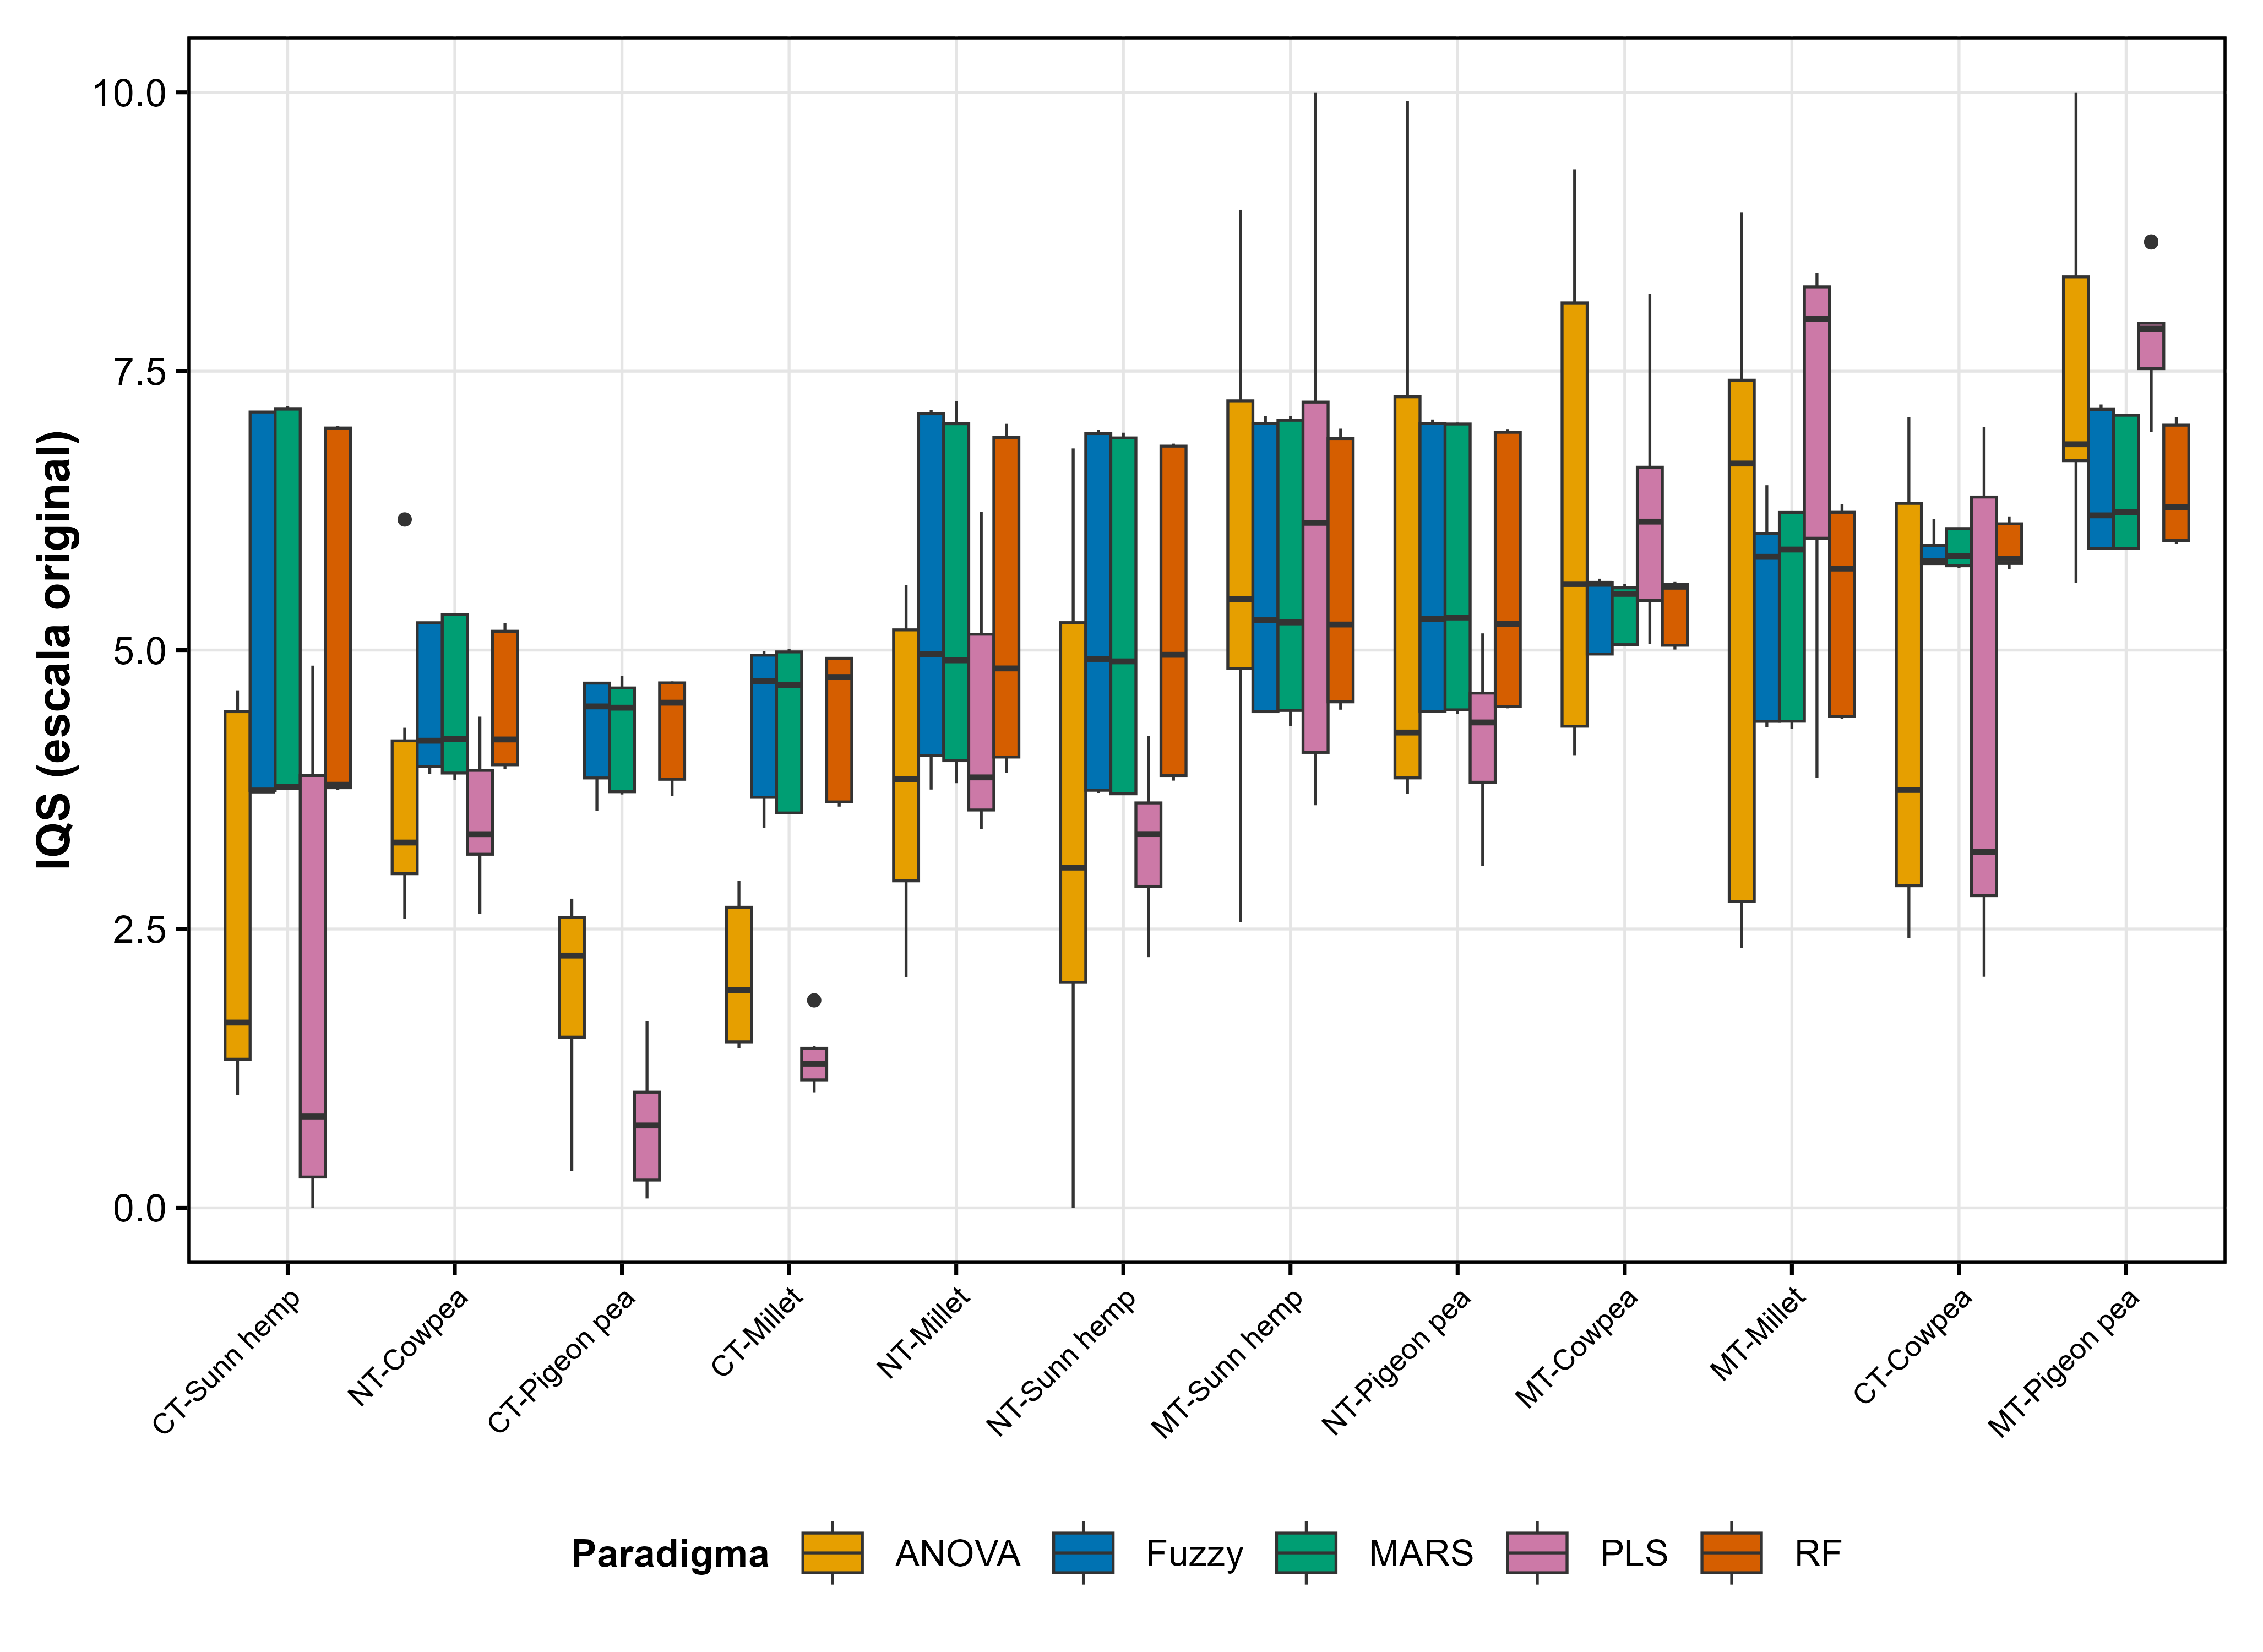
\includegraphics[width=\textwidth]{../../2-DADOS/3-FIGURAS/fig_boxplot_combo.png}
\caption{Distribuição do IQS (escala original, 0--10) por combinação manejo--cobertura e paradigma analítico.}\label{fig:boxplot_combo}
\smallskip\noindent\textit{Nota:} Combinações ordenadas pela média do meta-IQS de Borda.
\end{figure}

A superioridade do cultivo mínimo com guandu, já reportada por \cite{Assuncao2023} para o 17\textsuperscript{o} ano deste mesmo experimento, sugere persistência temporal do efeito de manejo ao longo de pelo menos cinco safras adicionais, configurando polaridade que pode refletir a interação entre a fixação biológica de nitrogênio do guandu e a magnitude do revolvimento mecânico aplicado. \cite{SantosJA2024}, ao avaliarem a produção de milho verde nas mesmas parcelas de longa duração no Nordeste brasileiro, observaram que o cultivo mínimo associado a plantas de cobertura produziu rendimentos 28\% superiores ao plantio convencional, com o guandu contribuindo para ruptura parcial da camada coesa pelo sistema radicular pivotante profundo ($> 2$~m). Esse mecanismo é consistente com observações de \cite{daSilva2021}, que verificaram em Argissolo Vermelho sob plantio direto que a sucessão milho/crotalária promoveu índice de estabilidade de agregados ($> 90$\%) superior à sucessão milho/pousio, atribuindo a diferença à glomalina e ao aporte contínuo de matéria orgânica particulada na rizosfera de leguminosas.

O posicionamento do plantio convencional com guandu na última posição de todos os cinco paradigmas (Borda\,=\,22,3) indica que o revolvimento intensivo anula os benefícios biológicos e agronômicos do guandu. \cite{Thomaz2022}, em experimento de 23 anos com tabaco no sul do Brasil, documentaram redução de 45\% no índice de estabilidade de agregados e incremento de erodibilidade ($K$-USLE de 0,018 para 0,031~Mg ha h ha$^{-1}$ MJ$^{-1}$ mm$^{-1}$) em plantio convencional comparado ao plantio direto, sugerindo que o revolvimento mecânico reiterado degrada progressivamente a estrutura do solo e sobrepõe-se ao efeito rizosférico da leguminosa. As posições intermediárias, contudo, apresentaram inversões entre paradigmas em 50\% das combinações manejo--cobertura (6 de 12). CM-Caupi ocupou a 2\textsuperscript{a} posição pela ANOVA, porém a 6\textsuperscript{a} por Fuzzy, MARS e RF, ao passo que PC-Caupi inverteu essa relação (2\textsuperscript{a} por Fuzzy/MARS/RF, 6\textsuperscript{a} por ANOVA). 

Essa inversão é consistente com a sensibilidade diferencial dos paradigmas à contribuição relativa dos indicadores físicos versus de rendimento, uma vez que o protocolo MDS da ANOVA aplica pesos derivados de ACP que equalizam domínios, enquanto os paradigmas não lineares ponderam pela capacidade preditiva estimada pelo algoritmo \cite{Chaudhry2024}. \cite{Fernandes2022}, em estudo sobre agregação em plantio direto com diferentes sucessões (milho/crotalária vs.\ milho/milheto vs.\ pousio), verificaram que a sucessão com leguminosa promoveu maior teor de carbono orgânico particulado e maior índice de estabilidade de agregados na camada 0--0,10~m, ao passo que a sucessão com gramínea favoreceu a macroporosidade subsuperficial (0,10--0,20~m). Essa diferenciação por profundidade e domínio pode explicar por que paradigmas que hierarquizam pela capacidade preditiva global (RF, MARS, SIF) ranqueiam caupi acima de milheto, enquanto a ANOVA, que equaliza pesos entre domínios físico e produtivo via ACP, inverte essa ordem. O PLS-SEM apresentou também divergências pontuais, colocando PD-Guandu em 6\textsuperscript{a} posição (contra 3\textsuperscript{a} nos demais), o que pode decorrer da exclusão de quatro indicadores por multicolinearidade na especificação do modelo estrutural. \cite{OliveiraFCC2024}, ao avaliarem frações oxidáveis de carbono orgânico do solo em Argissolo sob manejo conservacionista de longa duração no Nordeste brasileiro, observaram que o plantio direto com guandu acumulou maior proporção de carbono lábil (fração F1) na camada 0--0,05~m comparado aos demais sistemas, o que pode sensibilizar modelos não lineares que capturam relações entre frações de carbono e rendimento que o PLS-SEM, com menor dimensionalidade, não retém. Esses achados indicam que, para decisões de manejo baseadas em posições intermediárias do ranqueamento, a escolha do paradigma pode alterar a recomendação final, o que reforça a utilidade do meta-IQS de Borda como métrica de consenso \cite{Lin2010}. A quantificação ordinal consolidada dessas posições (Tabela~\ref{tab:ranking}) confirma a unanimidade nos extremos (CM-Guandu = 92,2; PC-Guandu = 22,3) e permite localizar cada inversão discutida.

\begin{table}[ht]
\caption{Ranqueamento das 12 combinações manejo--cobertura por cinco paradigmas e meta-IQS de Borda.}\label{tab:ranking}
\begin{tabular*}{\textwidth}{@{\extracolsep\fill}llcccccc}
\toprule
Manejo & Cobertura & ANOVA & Fuzzy & PLS & MARS & RF & Borda \\
\midrule
CM & Feijão-guandu & 1 & 1 & 1 & 1 & 1 & 92,2 \\
CM & Caupi         & 2 & 6 & 3 & 6 & 6 & 69,4 \\
CM & Milheto       & 4 & 5 & 2 & 5 & 5 & 69,0 \\
PC & Caupi         & 6 & 2 & 7 & 2 & 2 & 67,2 \\
CM & Crotalária    & 5 & 4 & 4 & 4 & 4 & 67,0 \\
PD & Feijão-guandu & 3 & 3 & 6 & 3 & 3 & 64,6 \\
PD & Milheto       & 7 & 7 & 5 & 7 & 7 & 55,7 \\
PD & Crotalária    & 9 & 8 & 9 & 8 & 8 & 46,4 \\
PD & Caupi         & 8 &10 & 8 &10 &10 & 38,6 \\
PC & Crotalária    &10 & 9 &10 & 9 & 9 & 35,4 \\
PC & Milheto       &11 &11 &11 &11 &11 & 26,3 \\
PC & Feijão-guandu &12 &12 &12 &12 &12 & 22,3 \\
\botrule
\end{tabular*}
\smallskip\noindent\textit{Nota:} PD, plantio direto; PC, plantio convencional; CM, cultivo mínimo. Valores de Borda mais elevados indicam melhor qualidade integrada do solo.
\end{table}

A unanimidade nos extremos da Tabela~\ref{tab:ranking} indica que a superioridade do cultivo mínimo com feijão-guandu e a inferioridade do plantio convencional com feijão-guandu são conclusões independentes do paradigma adotado, podendo ser incorporadas a recomendações agronômicas sem ressalva metodológica. Em contraste, qualquer recomendação envolvendo combinações situadas entre a 2\textsuperscript{a} e a 7\textsuperscript{a} posição deve ser acompanhada pela indicação explícita do paradigma utilizado e, preferencialmente, por análise de sensibilidade inter-paradigma que demonstre a estabilidade do posto atribuído. Essa prática de transparência metodológica é particularmente relevante em contextos de extensão rural e formulação de políticas públicas de conservação do solo, nos quais a indicação de um sistema de manejo pode mobilizar investimentos de longo prazo cujas consequências ultrapassam a incerteza estatística convencional.

\subsection{Sensibilidade ao tamanho amostral}\label{subsec:sensitivity_disc}

A concordância inter-paradigma cresceu com o tamanho amostral nas simulações Monte Carlo estratificadas, partindo de $\bar{W} = 0{,}683$ ($s = 0{,}167$) em $n = 15$ e atingindo $\bar{W} = 0{,}790$ ($s = 0{,}106$) em $n = 75$ (Fig.~\ref{fig:mc_box}). A dispersão de $W$ também se reduziu com o aumento de $n$, com o intervalo interquartílico contraindo de 0,22 ($n = 15$) para 0,08 ($n = 75$).

\begin{figure}[ht]
\centering
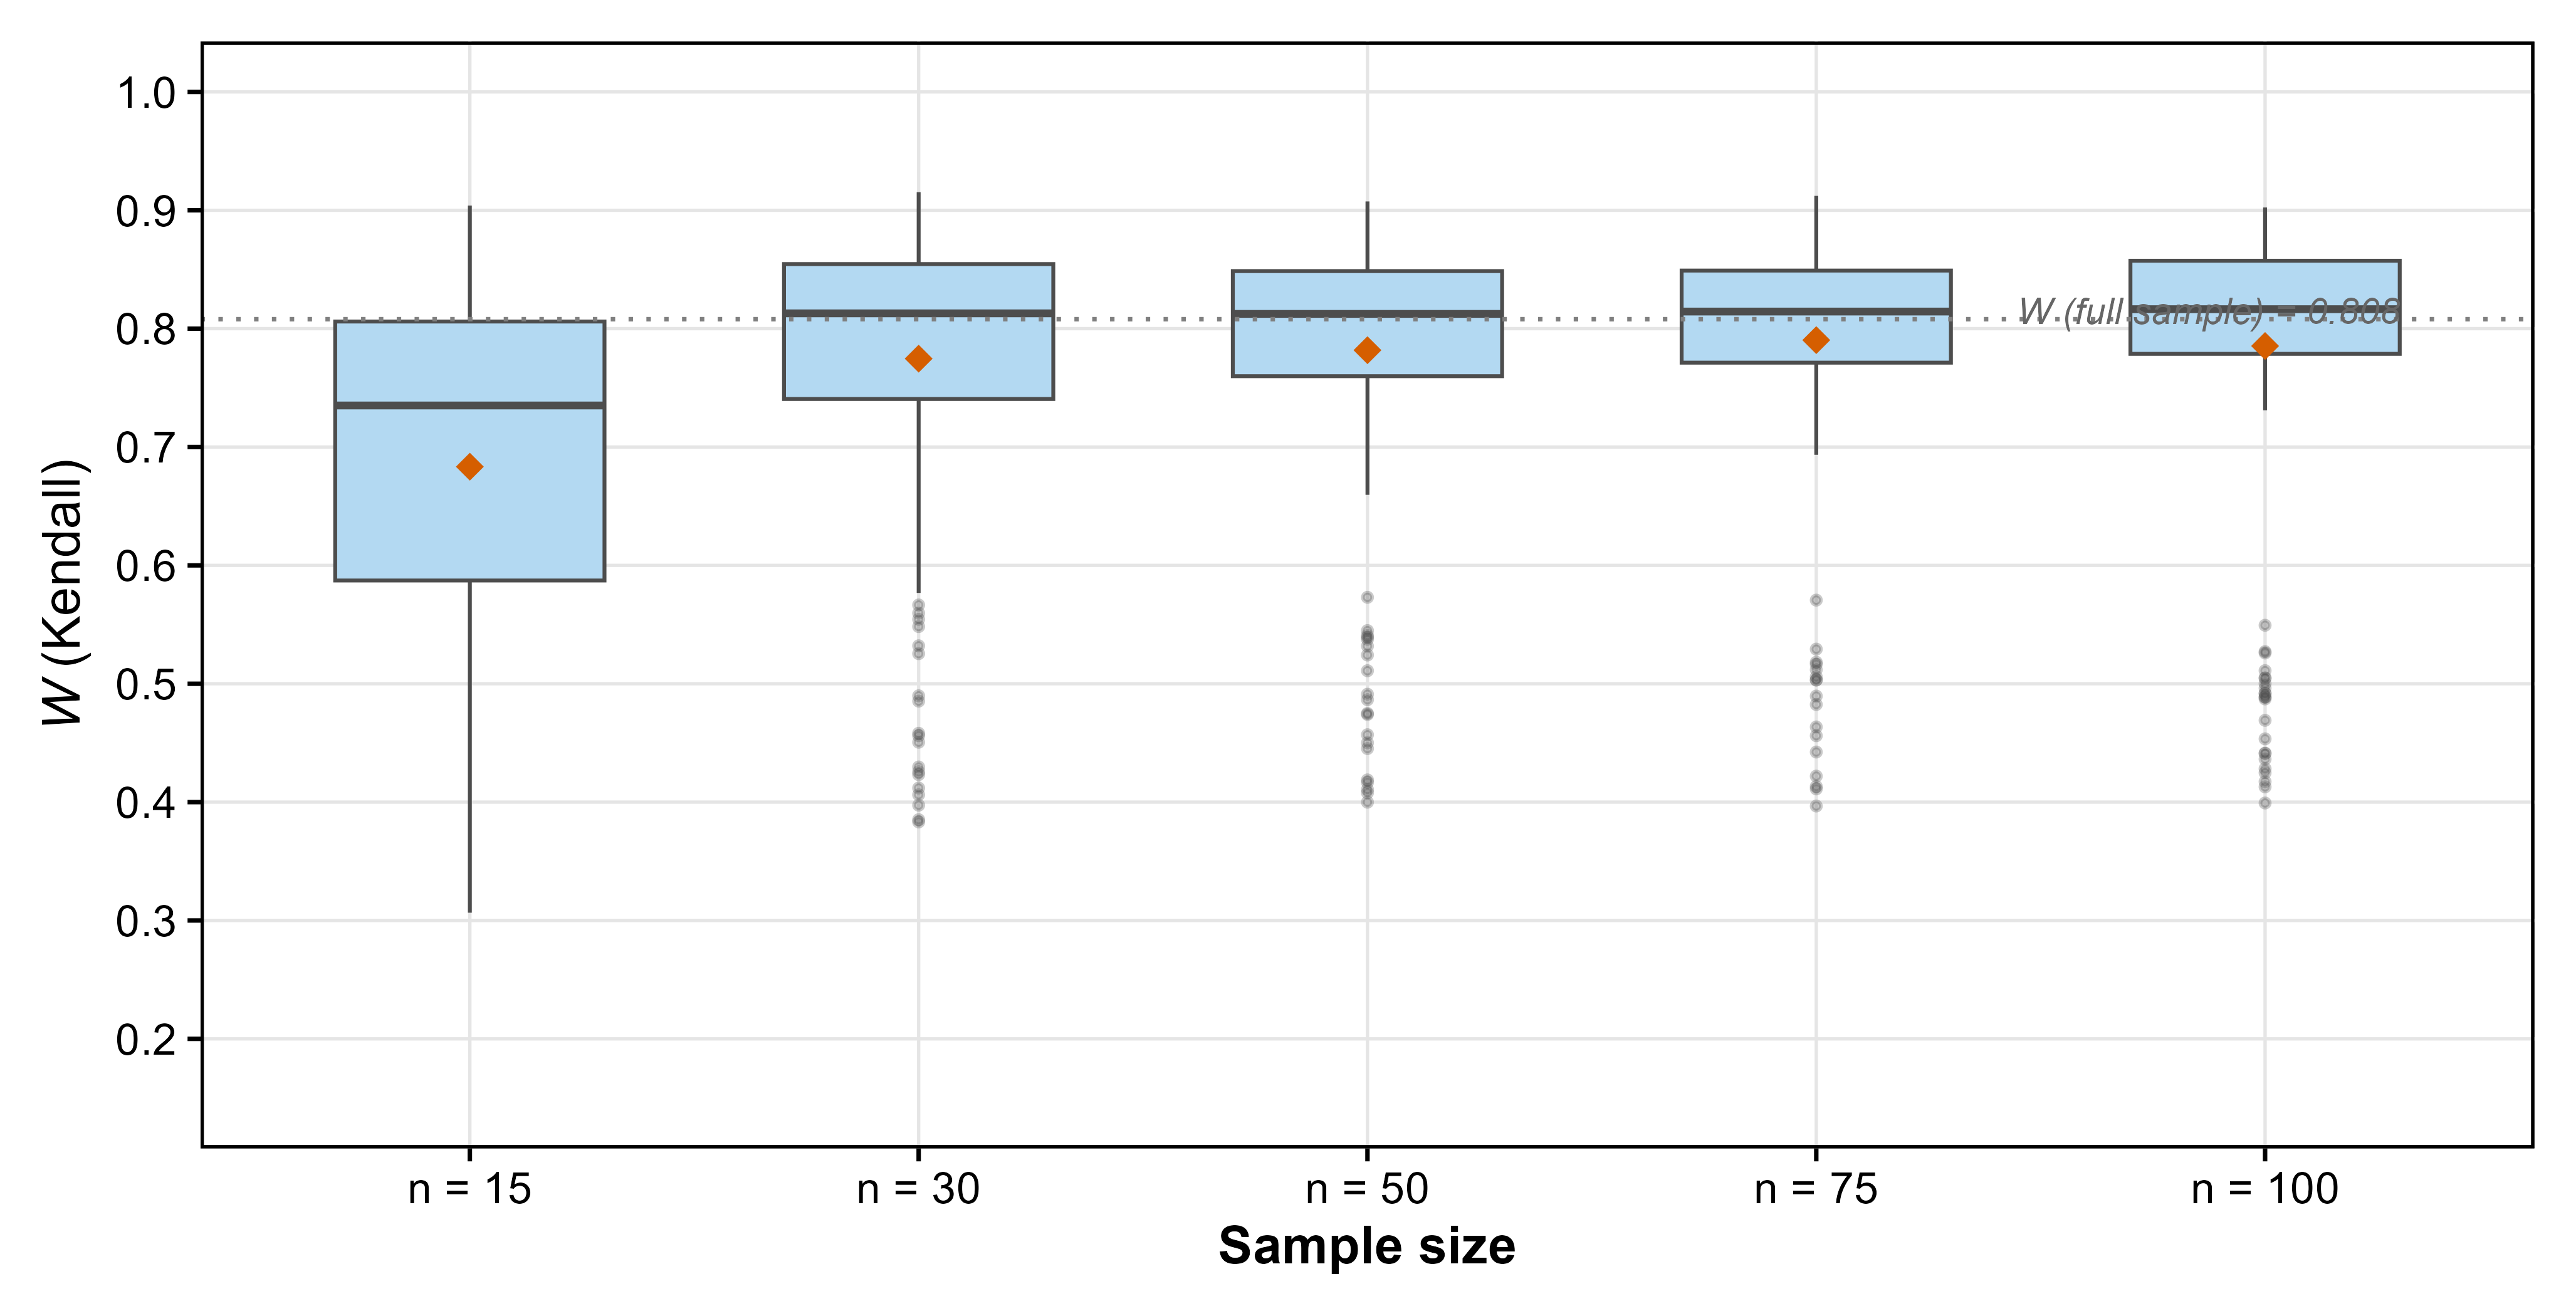
\includegraphics[width=0.75\textwidth]{../../2-DADOS/3-FIGURAS/fig_mc_sensitivity.png}
\caption{Distribuição do coeficiente de Kendall ($W$) em função do tamanho amostral ($n$), obtida por 200 iterações Monte Carlo estratificadas por célula do delineamento fatorial.}\label{fig:mc_box}
\smallskip\noindent\textit{Nota:} Losangos indicam a média; linha pontilhada indica $W$ da amostra completa ($n = 108$).
\end{figure}

Em $n = 100$, $\bar{W}$ recuou ligeiramente para 0,785 ($s = 0{,}120$), sugerindo estabilização a partir de $n \approx 50$. A reta GLS ajustada sobre $\log(n)$ indicou tendência positiva ($\hat{\beta}_1 = 0{,}043$), embora o efeito não tenha atingido significância convencional ($p = 0{,}098$), e a faixa de percentis 2,5--97,5\% convergiu progressivamente para a referência da amostra completa.

Essa marginalidade pode refletir o número reduzido de níveis amostrais ($k = 5$), que limita a potência estatística do teste \cite{Mundform2005}. \cite{Adak2023}, ao aplicarem IQS sob manejos contrastantes de preparo, resíduo e nitrogênio em rotação milho--trigo na planície Indo-Gangética, verificaram que amostras com $n < 30$ inflaram a incerteza dos pesos derivados de ACP, desestabilizando o ranqueamento dos tratamentos e produzindo inversões de posição entre manejos que, com a amostra completa ($n = 96$), eram estatisticamente distintos. Amostras menores aumentam a discrepância estocástica na estimativa de postos, separando artificialmente paradigmas que convergiriam com amostras maiores. Exercícios de \textit{benchmarking} com $n < 30$ podem produzir comparações instáveis ($\bar{W} < 0{,}78$, $s > 0{,}12$), ao passo que $n \geq 50$ parece suficiente para estabilizar a concordância.

\subsection{Implicações para monitoramento e transferibilidade}\label{subsec:implications}

Quando o interesse recai sobre ranqueamento de combinações manejo--cobertura em bases com $n \geq 50$, qualquer representante do bloco não linear (SIF, MARS ou RF) pode ser adotado com diferenças negligenciáveis ($\rho > 0{,}99$), dispensando análise de sensibilidade ao paradigma. Se a interpretabilidade dos caminhos causais entre domínios edáficos for prioritária, conforme recomendado em avaliações de indicadores compostos \cite{Cardoso2013}, o PLS-SEM oferece alternativa com divergência moderada em relação ao bloco não linear (LoA\,$\approx \pm 1{,}65$), embora a exclusão de indicadores por multicolinearidade possa comprometer a representatividade do domínio físico. O paradigma ANOVA/MDS permanece útil para compatibilidade com o extenso acervo de estudos que adotaram o protocolo de \cite{Andrews2002} e para bases com número reduzido de indicadores ($p < 10$), condição na qual vantagens de métodos não lineares tendem a ser marginais \cite{Bünemann2018}. Esse protocolo de seleção, esquematizado no Apêndice~\ref{secA1}, pode servir como referência para pesquisadores e extensionistas que necessitem justificar a escolha metodológica em avaliações de qualidade do solo.

A generalização destes achados requer cautela. Os dados provêm de experimento conduzido sobre Argissolo com camada coesa \cite{LimaNeto2010} sob clima As$'$, condição na qual relações não lineares entre indicadores podem ser acentuadas pelo impedimento físico subsuperficial. Solos sem restrição física, ou sistemas com menor diversidade de práticas, poderiam exibir concordância inter-paradigma mais elevada, reduzindo a diferenciação entre famílias analíticas. \cite{Zhao2022}, em solo negro submetido a 19 anos de manejo conservacionista na China, verificaram que atributos físicos (estabilidade de agregados, porosidade) foram mais sensíveis ao tipo de preparo do que indicadores químicos, os quais responderam predominantemente à adubação. Em solos tropicais com camada coesa, a contribuição dos atributos físicos para o IQS tende a ser comprimida pela baixa diferenciação espacial na profundidade amostrada, o que pode amplificar a divergência entre paradigmas que competem por variância explicável em poucos indicadores físicos. A aplicação deste mesmo \textit{framework} a bases provenientes de outras classes de solo e regiões climáticas é uma direção promissora para investigações futuras, particularmente em Latossolos argilosos do Cerrado, onde \cite{DosSantos2021} já demonstraram a eficácia do IQS fuzzy na diferenciação entre sistemas de cobertura.

Algumas limitações merecem menção. O PLS-SEM utilizou 11 dos 15 indicadores originais após exclusão de quatro variáveis por multicolinearidade (VIF\,$> 5$), o que pode subestimar a contribuição do domínio físico. A simulação Monte Carlo empregou 200 iterações com reamostragem do mesmo conjunto de dados, preservando a estrutura de correlação original sem substituir validação externa. A classificação do PLS-SEM como ``não linear'' em $H_2$ é discutível, dado que o modelo especifica caminhos lineares entre construtos; uma reclassificação como ``misto'' fortaleceria a distinção entre paradigmas puramente não lineares e o paradigma linear.

%% ================================================================
%%                    SEÇÃO 5: CONCLUSÃO
%% ================================================================
\section{Conclusão}\label{sec:conclusion}

A concordância inter-paradigma foi significativa ($W = 0{,}81$), confirmando $H_1$, porém distribuiu-se em três camadas de intensidade que sustentam $H_2$: SIF, MARS e RF são mutuamente substituíveis (30\% dos pares, $\rho > 0{,}99$, LoA\,$< \pm 0{,}50$), o PLS-SEM diverge moderadamente (30\% dos pares, LoA\,$\approx \pm 1{,}65$) e a ANOVA pode inverter posições intermediárias de manejo (40\% dos pares, LoA\,$> \pm 1{,}85$). A concordância estabilizou acima de $n \approx 50$, oferecendo suporte parcial a $H_3$. Esses limiares de substituibilidade podem orientar a seleção de paradigma em avaliações de IQS, embora sua generalização a outras classes de solo e regimes climáticos requeira validação externa.

\backmatter

\bmhead{Informação suplementar}

Todas as rotinas R e Python utilizadas neste estudo, bem como o conjunto de dados anonimizado, encontram-se disponíveis em [URL DO REPOSITÓRIO]. As Tabelas Suplementares S1--S4 apresentam a saída completa da ANOVA, a base de regras fuzzy, os coeficientes de caminho do PLS-SEM e os ranqueamentos de importância de variáveis.

\bmhead{Agradecimentos}

%% [A COMPLETAR]

\section*{Declarações}

\begin{itemize}
\item \textbf{Financiamento:} [A COMPLETAR]
\item \textbf{Conflito de interesses:} Os autores declaram não possuir interesses concorrentes.
\item \textbf{Aprovação ética:} Não aplicável.
\item \textbf{Consentimento para publicação:} Não aplicável.
\item \textbf{Disponibilidade de dados:} O conjunto de dados e o código que sustentam este estudo encontram-se disponíveis em [URL DO REPOSITÓRIO].
\item \textbf{Disponibilidade de código:} Todas as rotinas de análise (R e Python) encontram-se disponíveis em [URL DO REPOSITÓRIO].
\item \textbf{Contribuição dos autores:} [A COMPLETAR]
\end{itemize}

\begin{appendices}

\section{Fluxograma decisório para seleção de paradigma}\label{secA1}

%% [Fluxograma TikZ A INSERIR]

\section{Base de regras fuzzy completa}\label{secA2}

%% [A INSERIR]

\section{Coeficientes de caminho PLS-SEM e diagnósticos}\label{secA3}

%% [A INSERIR]

\end{appendices}

\bibliography{sn-bibliography}% common bib file

\end{document}
